% Elaborado por Fabian Gomez
% Version 1.0

\section{System Architecture and Model References}\label{sec:architecture}

Esta sección establece los límites técnicos y las decisiones de diseño de alto nivel que actúan como restricciones mandatorias para el desarrollo del Rover Olympus. La arquitectura se organiza en siete subsistemas principales, siguiendo estándares internacionales de ingeniería de sistemas espaciales (NASA/JPL) para asegurar una clara separación de funciones entre locomoción, actuación y control.

\subsection{Vista Funcional del Sistema}\label{subsec:functional_view}

Esta vista describe la organización lógica de las capacidades del Rover Olympus y cómo se distribuyen las responsabilidades operacionales antes de su asignación a componentes físicos de hardware.

\subsubsection{Block Definition Diagram (BDD) -- Arquitectura de Subsistemas}

El BDD del sistema \textit{Rover Olympus} define la descomposición estructural a nivel de arquitectura de sistema, representando al rover como un bloque principal compuesto por siete subsistemas. La relación principal usada es \textbf{composición} (\textit{part-of}), indicando que cada subsistema es una parte constitutiva del rover y que su integración es necesaria para lograr las capacidades del sistema (movilidad, energía, cómputo a bordo, comunicaciones, navegación y soporte mecánico).


\begin{landscape}
\begin{figure}[H]
    \centering
    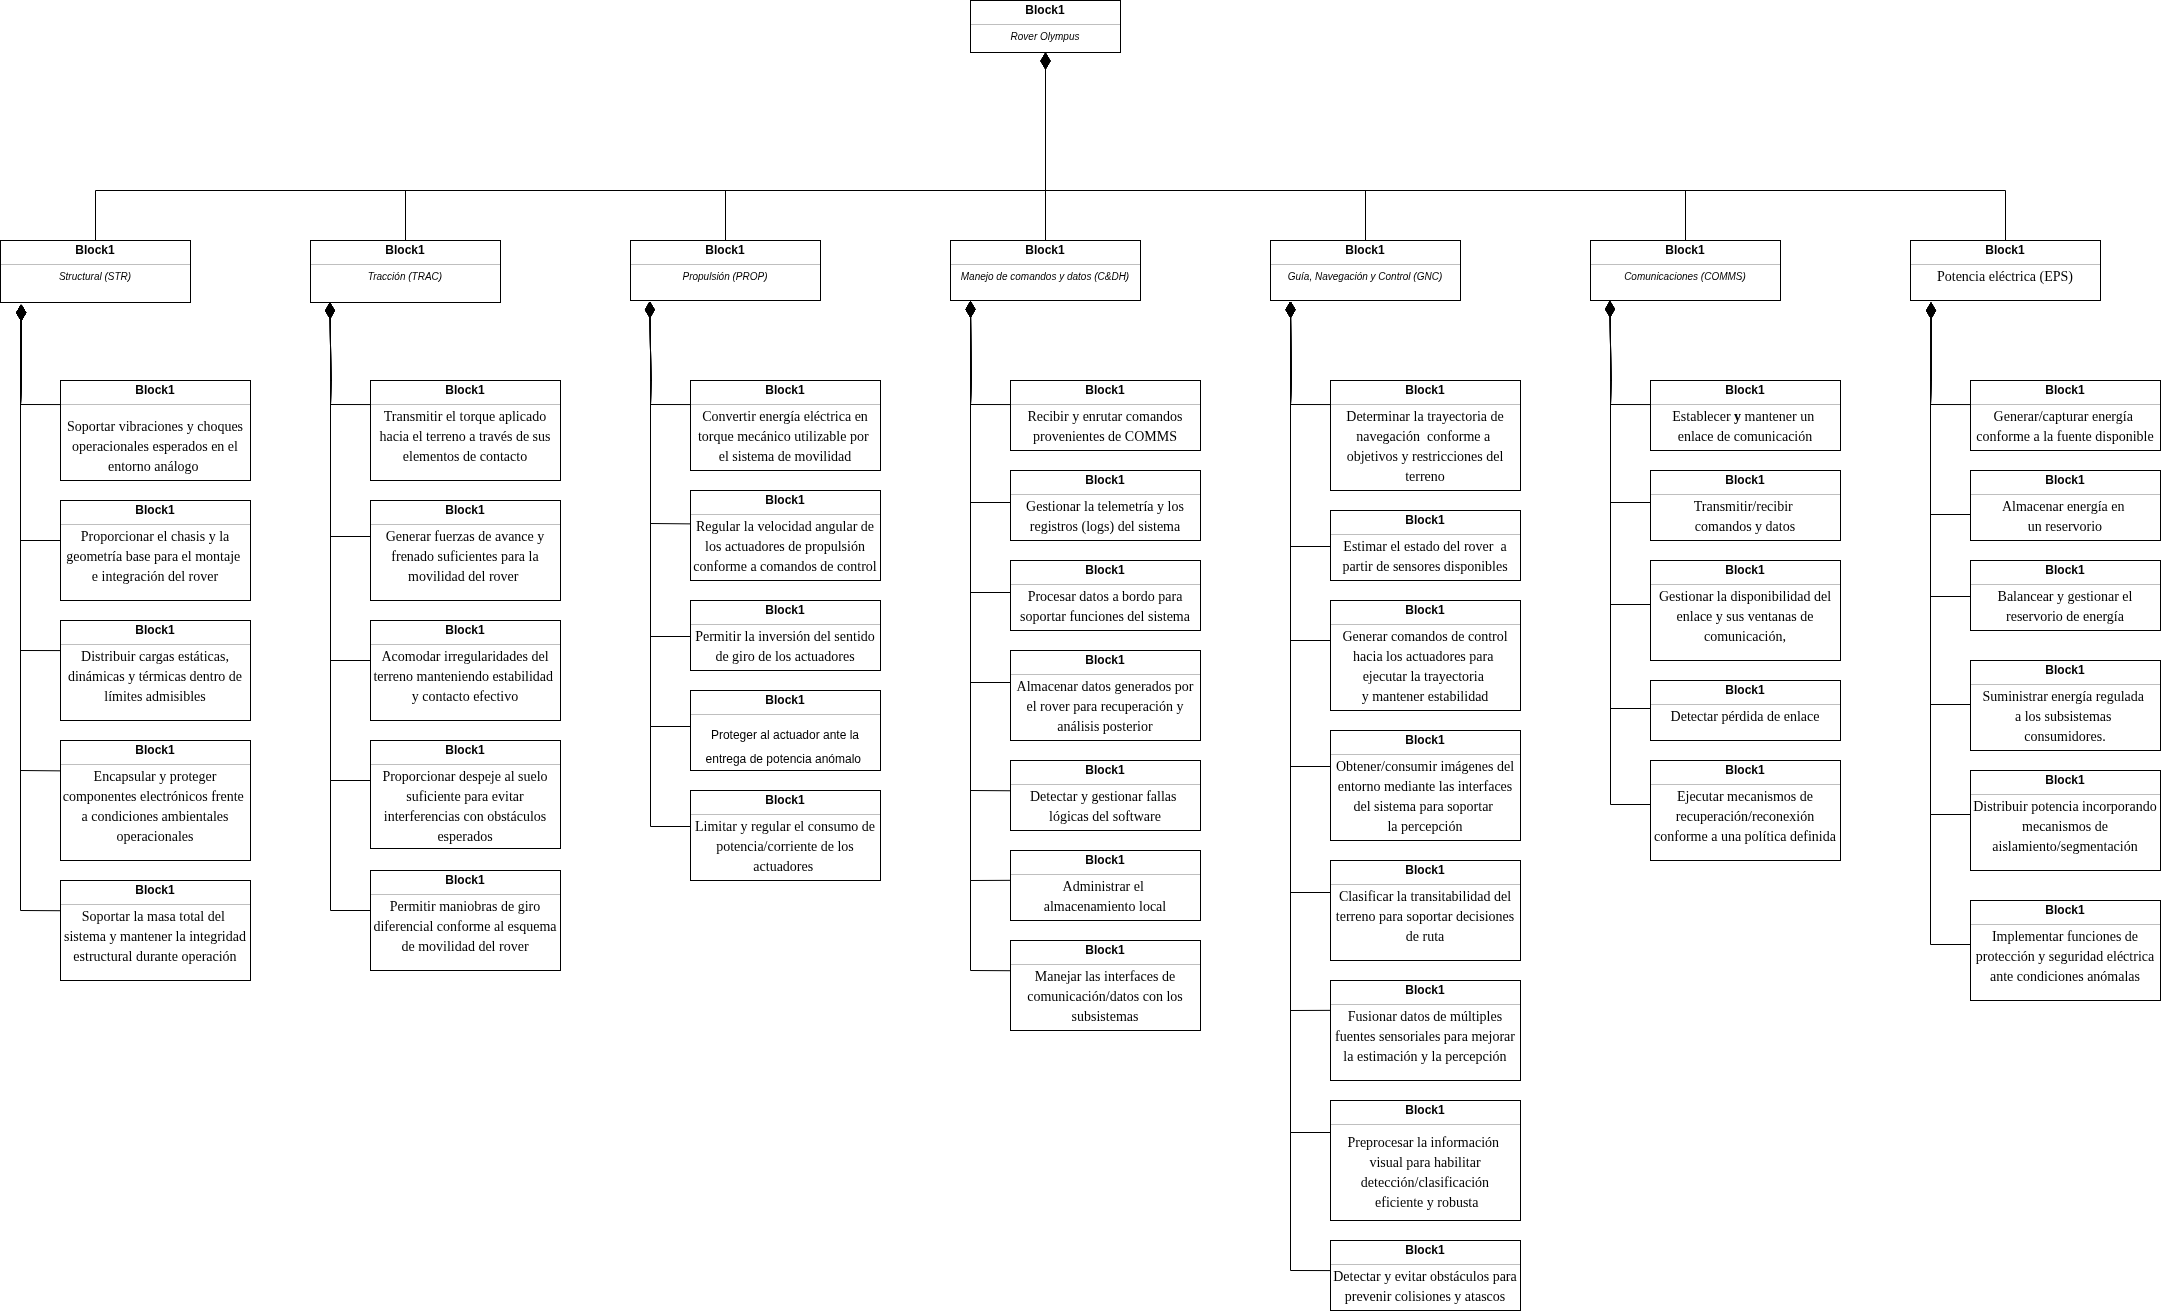
\includegraphics[width=0.7\paperheight]{figures/BDD-bdd.drawio.png}
    \caption{Block Definition Diagram (BDD) -- Jerarquía lógica de los 7 subsistemas.}
    \label{fig:paso1}
\end{figure}
\end{landscape}


\paragraph{Bloque principal: Rover Olympus.}
El bloque \texttt{Rover\_Olympus} encapsula la arquitectura del rover y agrupa los siete subsistemas: \texttt{Structural}, \texttt{TRAC}, \texttt{PROP}, \texttt{EPS}, \texttt{C\&DH}, \texttt{GNC} y \texttt{COMMS}. Esta partición es coherente con una descomposición funcional típica de rovers de exploración, separando (i) la movilidad en conversión electro-mecánica (PROP) e interacción terreno (TRAC), (ii) la energía (EPS), (iii) el cómputo y manejo de datos (C\&DH), (iv) la navegación/autonomía (GNC), (v) el enlace con estación base (COMMS), y (vi) la estructura mecánica (Structural).

\paragraph{Relaciones e interfaces conceptuales entre subsistemas (nivel arquitectura).}
A nivel de BDD se representan asociaciones conceptuales que orientan las interfaces del sistema:
(i) \texttt{EPS} se asocia con todos los subsistemas consumidores de potencia (distribución/energía);
(ii) \texttt{COMMS} se asocia con \texttt{C\&DH} como canal de comandos y telemetría;
(iii) \texttt{C\&DH} se asocia con los subsistemas para gestión de datos, telemetría e interfaces;
(iv) \texttt{GNC} se asocia con \texttt{PROP} y \texttt{TRAC} para generación de comandos de movilidad, y con \texttt{C\&DH} para ejecución/orquestación y registro de datos.

El BDD no detalla diseño electrónico ni componentes; su propósito es fijar la estructura de alto nivel y soportar trazabilidad de requisitos e interfaces entre subsistemas.


\subsubsection{Mapeo de Funciones de los Subsistemas por componentes (PBS)}

\begin{landscape}
\scriptsize
\renewcommand{\arraystretch}{1.15}
\setlength{\tabcolsep}{3pt}
\begin{longtable}{|p{0.9cm}|p{2.0cm}|p{6.8cm}|p{9.2cm}|}
\caption{Funciones del BDD vs. Componentes COTS propuestos (tabla reducida)}\label{tab:funciones_cots_reducida}\\
\hline
\textbf{ID} & \textbf{Subsistema / Bloque} & \textbf{Nombre de la función} & \textbf{Componente(s) COTS propuesto(s)}\\
\hline
\endfirsthead

\hline
\textbf{ID} & \textbf{Subsistema / Bloque} & \textbf{Nombre de la función} & \textbf{Componente(s) COTS propuesto(s)}\\
\hline
\endhead

\hline
\multicolumn{4}{r}{\textit{Continúa en la siguiente página}}\\
\endfoot

\hline
\endlastfoot

% -------------------- STR --------------------
F1 & STR & Soportar vibraciones y choques operacionales esperados en el entorno análogo &
Estructura impresa (PLA MAX) + aisladores/soportes antivibración + tornillería/inserciones.\\ \hline

F2 & STR & Proporcionar el chasis y la geometría base para el montaje e integración del rover &
Chasis modular impreso (PLA MAX) + perfiles/placas de refuerzo (si aplica).\\ \hline

F3 & STR & Distribuir cargas estáticas, dinámicas y térmicas dentro de límites admisibles &
Estructura con refuerzos + separadores/insertos roscados + uniones mecánicas.\\ \hline

F4 & STR & Encapsular y proteger componentes electrónicos frente a condiciones ambientales operacionales &
Caja/electronics bay impresa (PLA MAX) + prensaestopas/juntas (si aplica).\\ \hline

F5 & STR & Soportar la masa total del sistema y mantener la integridad estructural durante operación &
Chasis reforzado + distribución de masa + puntos de montaje/agarre.\\ \hline

% -------------------- TRAC --------------------
F6 & TRAC & Transmitir el torque aplicado hacia el terreno a través de sus elementos de contacto &
Ruedas/llantas + hubs impresos (PLA MAX) + rodamientos F687ZZ + ejes/acoples.\\ \hline

F7 & TRAC & Generar fuerzas de avance y frenado suficientes para la movilidad del rover &
Motores DC (NFP-5840-31ZY-EN) + ruedas/llantas + control PWM mediante drivers.\\ \hline

F8 & TRAC & Acomodar irregularidades del terreno manteniendo estabilidad y contacto efectivo &
Suspensión pasiva (bogies/rocker simple) + articulaciones con rodamientos + piezas impresas.\\ \hline

F9 & TRAC & Proporcionar despeje al suelo suficiente para evitar interferencias con obstáculos esperados &
Selección de diámetro de rueda + geometría de chasis + posible suspensión (diseño mecánico).\\ \hline

F10 & TRAC & Proporcionar capacidad de dirección (steering) y maniobra conforme al esquema de movilidad &
Control de motores (skid-steer) y servomotor de dirección (MG996R) mediante Arduino Mega.\\ \hline

% -------------------- PROP --------------------
F11 & PROP & Convertir energía eléctrica en torque mecánico utilizable por el sistema de movilidad &
Motores DC con reductora (NFP-5840-31ZY-EN) + acoples a rueda/tren de tracción.\\ \hline

F12 & PROP & Regular la velocidad angular de los actuadores de propulsión conforme a comandos de control &
Drivers mixtos (L298N para motores frontales FR/FL; BTS7960 para CR/CL/RR/RL) con PWM + Arduino Mega (control en tiempo real) + Raspberry Pi 5 (alto nivel vía UART).\\ \hline

F13 & PROP & Permitir la inversión del sentido de giro de los actuadores &
Drivers mixtos (L298N + BTS7960) + control digital desde Arduino Mega.\\ \hline

F14 & PROP & Proteger al actuador ante la entrega de potencia anómala &
Protecciones por canal (L298N + BTS7960) + ACS712 por motor (disparo \texttt{OC\_FAULT} en LLC) + INA3221 (3 bancos, telemetría tensión) + fusibles/TVS por rama. No se emplea BMS centralizado en la arquitectura desplegada.\\ \hline

F15 & PROP & Limitar y regular el consumo de potencia/corriente de los actuadores &
Drivers mixtos (L298N + BTS7960) + control (Arduino Mega) + sensado de corriente implementado (ACS712 por motor + INA3221 3 bancos en modo bus-only).\\ \hline

% -------------------- C&DH --------------------
F16 & C\&DH & Recibir y enrutar comandos provenientes de COMMS &
Raspberry Pi 4/5 (interfaz de red y ruteo de comandos) + enlace (Wi-Fi/radio).\\ \hline

F17 & C\&DH & Gestionar la telemetría y los registros (logs) del sistema &
Raspberry Pi 4/5 + almacenamiento local (microSD/SSD) + software de logging.\\ \hline

F18 & C\&DH & Procesar datos a bordo para soportar funciones del sistema &
Raspberry Pi 5 (única OBC desplegada; arquitectura single-node sin redundancia activa de cómputo).\\ \hline

F19 & C\&DH & Almacenar datos generados por el rover para recuperación y análisis posterior &
Almacenamiento local (microSD/SSD) conectado a Raspberry Pi 4/5.\\ \hline

F20 & C\&DH & Detectar y gestionar fallas lógicas del software &
Watchdog SW/HW en Raspberry Pi + (opcional) Arduino Mega como supervisor auxiliar.\\ \hline

F21 & C\&DH & Administrar el almacenamiento local &
Raspberry Pi 4/5 + gestión de filesystem/rotación de logs (software).\\ \hline

F22 & C\&DH & Manejar las interfaces de comunicación/datos con los subsistemas &
Arduino Mega (I/O y tiempo real) + Raspberry Pi 4/5 (alto nivel) + buses (UART/I2C/SPI/USB).\\ \hline

% -------------------- GNC --------------------
F23 & GNC & Determinar la trayectoria de navegación conforme a objetivos y restricciones del terreno &
Raspberry Pi 4/5 (planificación) + (recomendado) sensores de navegación (IMU/odometría/LiDAR).\\ \hline

F24 & GNC & Estimar el estado del rover a partir de sensores disponibles &
Raspberry Pi 4/5 + fusión sensorial (EKF) + (recomendado) IMU + encoders (si disponibles).\\ \hline

F25 & GNC & Generar comandos de control hacia los actuadores para ejecutar la trayectoria y mantener estabilidad &
Arduino Mega (control) + drivers mixtos (L298N + BTS7960) + motores DC + \texttt{QuadratureEncoder} por rueda (lazo cerrado \texttt{MotorWithEncoder}, LLC v2.20).\\ \hline

F26 & GNC & Obtener/consumir imágenes del entorno mediante las interfaces del sistema para soportar la percepción &
Cámara CSI \textbf{OV5647} (sensor RPi Cam v1.3) + Raspberry Pi 5. (Canal FPV 5.8\,GHz independiente para monitoreo humano; no consumido por el pipeline GNC.)\\ \hline

F27 & GNC & Preprocesar la información visual para habilitar detección/clasificación eficiente y robusta &
Raspberry Pi 5 + pipeline de visión (OpenCV + YOLOv8n-seg) + cámara OV5647.\\ \hline

F28 & GNC & Detectar y evitar obstáculos para prevenir colisiones y atascos &
OV5647 + RPi5 (visión YOLOv8n-seg) + \textbf{LiDAR TF02} (UART, rango táctico) + \textbf{VL53L0X} ToF (I2C, corte emergencia LLC $\le$200\,mm) + \textbf{HC-SR04} ultrasonido (GPIO LLC, redundancia).\\ \hline

F29 & GNC & Fusionar datos de múltiples fuentes sensoriales para mejorar la estimación y la percepción &
Raspberry Pi 5 + fusión (TBD futuro EKF/UKF) + \textbf{MPU-6050} IMU (I2C) + encoders cuadratura + rango (TF02/VL53L0X/HC-SR04) + visión (OV5647).\\ \hline

F30 & GNC & Clasificar la transitabilidad del terreno para soportar decisiones de ruta &
Raspberry Pi 5 + cámara OV5647 (clasificación por visión: YOLOv8n-seg COCO baseline; pendiente fine-tuning terreno volcánico --- RF-002).\\ \hline

% -------------------- COMMS --------------------
F31 & COMMS & Establecer y mantener un enlace de comunicación &
Raspberry Pi 4/5 (Wi-Fi) + enlace FPV (TX/RX) para video.\\ \hline

F32 & COMMS & Transmitir/recibir comandos y datos &
Raspberry Pi 4/5 (Wi-Fi/protocolo) + (opcional) radio telemetría externa.\\ \hline

F33 & COMMS & Gestionar la disponibilidad del enlace y sus ventanas de comunicación, &
Raspberry Pi 4/5 (supervisión de enlace, QoS, reconexión) + infraestructura de red.\\ \hline

F34 & COMMS & Detectar pérdida de enlace &
Raspberry Pi 4/5 (heartbeat/timeouts) + política fail-safe (software).\\ \hline

% -------------------- EPS --------------------
F35 & EPS & Generar/capturar energía conforme a la fuente disponible &
Bancos de 18650 NMC + cargador externo de Li-ion (sin generación propia a bordo; integración fotovoltaica diferida como trabajo futuro).\\ \hline

F36 & EPS & Almacenar energía en un reservorio &
Arquitectura de \textbf{3 bancos} 18650 NMC (rail principal + 2 rails secundarios), con telemetría de tensión por INA3221 (un canal por banco).\\ \hline

F37 & EPS & Balancear y gestionar el reservorio de energía &
Protecciones por banco (fusibles + ACS712 + supervisión INA3221). No se emplea BMS centralizado en la arquitectura desplegada (decisión de diseño 2026-05-17, ver memoria \texttt{session\_2026\_05\_17\_ina3221}); el balanceo manual se realiza fuera del rover durante la carga.\\ \hline

F38 & EPS & Suministrar energía regulada a los subsistemas consumidores. &
Convertidores DC-DC (buck 3 bancos $\rightarrow$ 5\,V / 12\,V según cargas) + distribución por PDU.\\ \hline

F39 & EPS & Distribuir potencia incorporando mecanismos de aislamiento/segmentación &
Power Distribution Unit (PDU) + fusibles por rama + relay de corte de emergencia (\texttt{BNK:0}) accionable por GCS via ICD-LLC-001.\\ \hline

F40 & EPS & Implementar funciones de protección y seguridad eléctrica ante condiciones anómalas &
Fusibles por banco + ACS712 por motor (disparo \texttt{OC\_FAULT} en LLC) + INA3221 (telemetría tensión) + e-stop relay \texttt{BNK:0} + buenas prácticas de cableado.\\ \hline

F41 & EPS & Ejecutar mecanismos de recuperación/reconexión conforme a una política definida &
Raspberry Pi 4/5 + (opcional) relé/contactor + supervisor de tensión (según política).\\ \hline

\end{longtable}
\end{landscape}
\subsubsection{Behavioral and Parametric References}

Los modelos de comportamiento (Casos de Uso, Actividad y Estados) y los modelos paramétricos se enlazan a la arquitectura de 7 subsistemas para verificar el cumplimiento de los RNF de desempeño y las restricciones de misión. \cite{segoldmine_ppi, nasa_cm}


\subsection{Arquitectura Física del Sistema}\label{subsec:physical_view}

Esta vista detalla la implementación del sistema mediante componentes de hardware COTS y define cómo se integran físicamente para cumplir con la vista funcional.

\subsubsection{Descripción por subsistemas (IBD físico) del Rover Olympus}
Una vez definidos el sistema \textit{Rover Olympus} y sus elementos físicos, se construye la arquitectura física mediante un \textbf{Internal Block Diagram (IBD)}. En este diagrama se \textbf{mapean explícitamente} los componentes de hardware a las funciones del modelo funcional, y se detallan las \textbf{interfaces} (potencia, datos, control, RF y mecánicas) que habilitan las interacciones entre subsistemas. A continuación, se describe la interacción del sistema por subsistemas, considerando los componentes internos modelados y sus conexiones principales. 

\begin{landscape}
\begin{figure}[H]
    \centering
    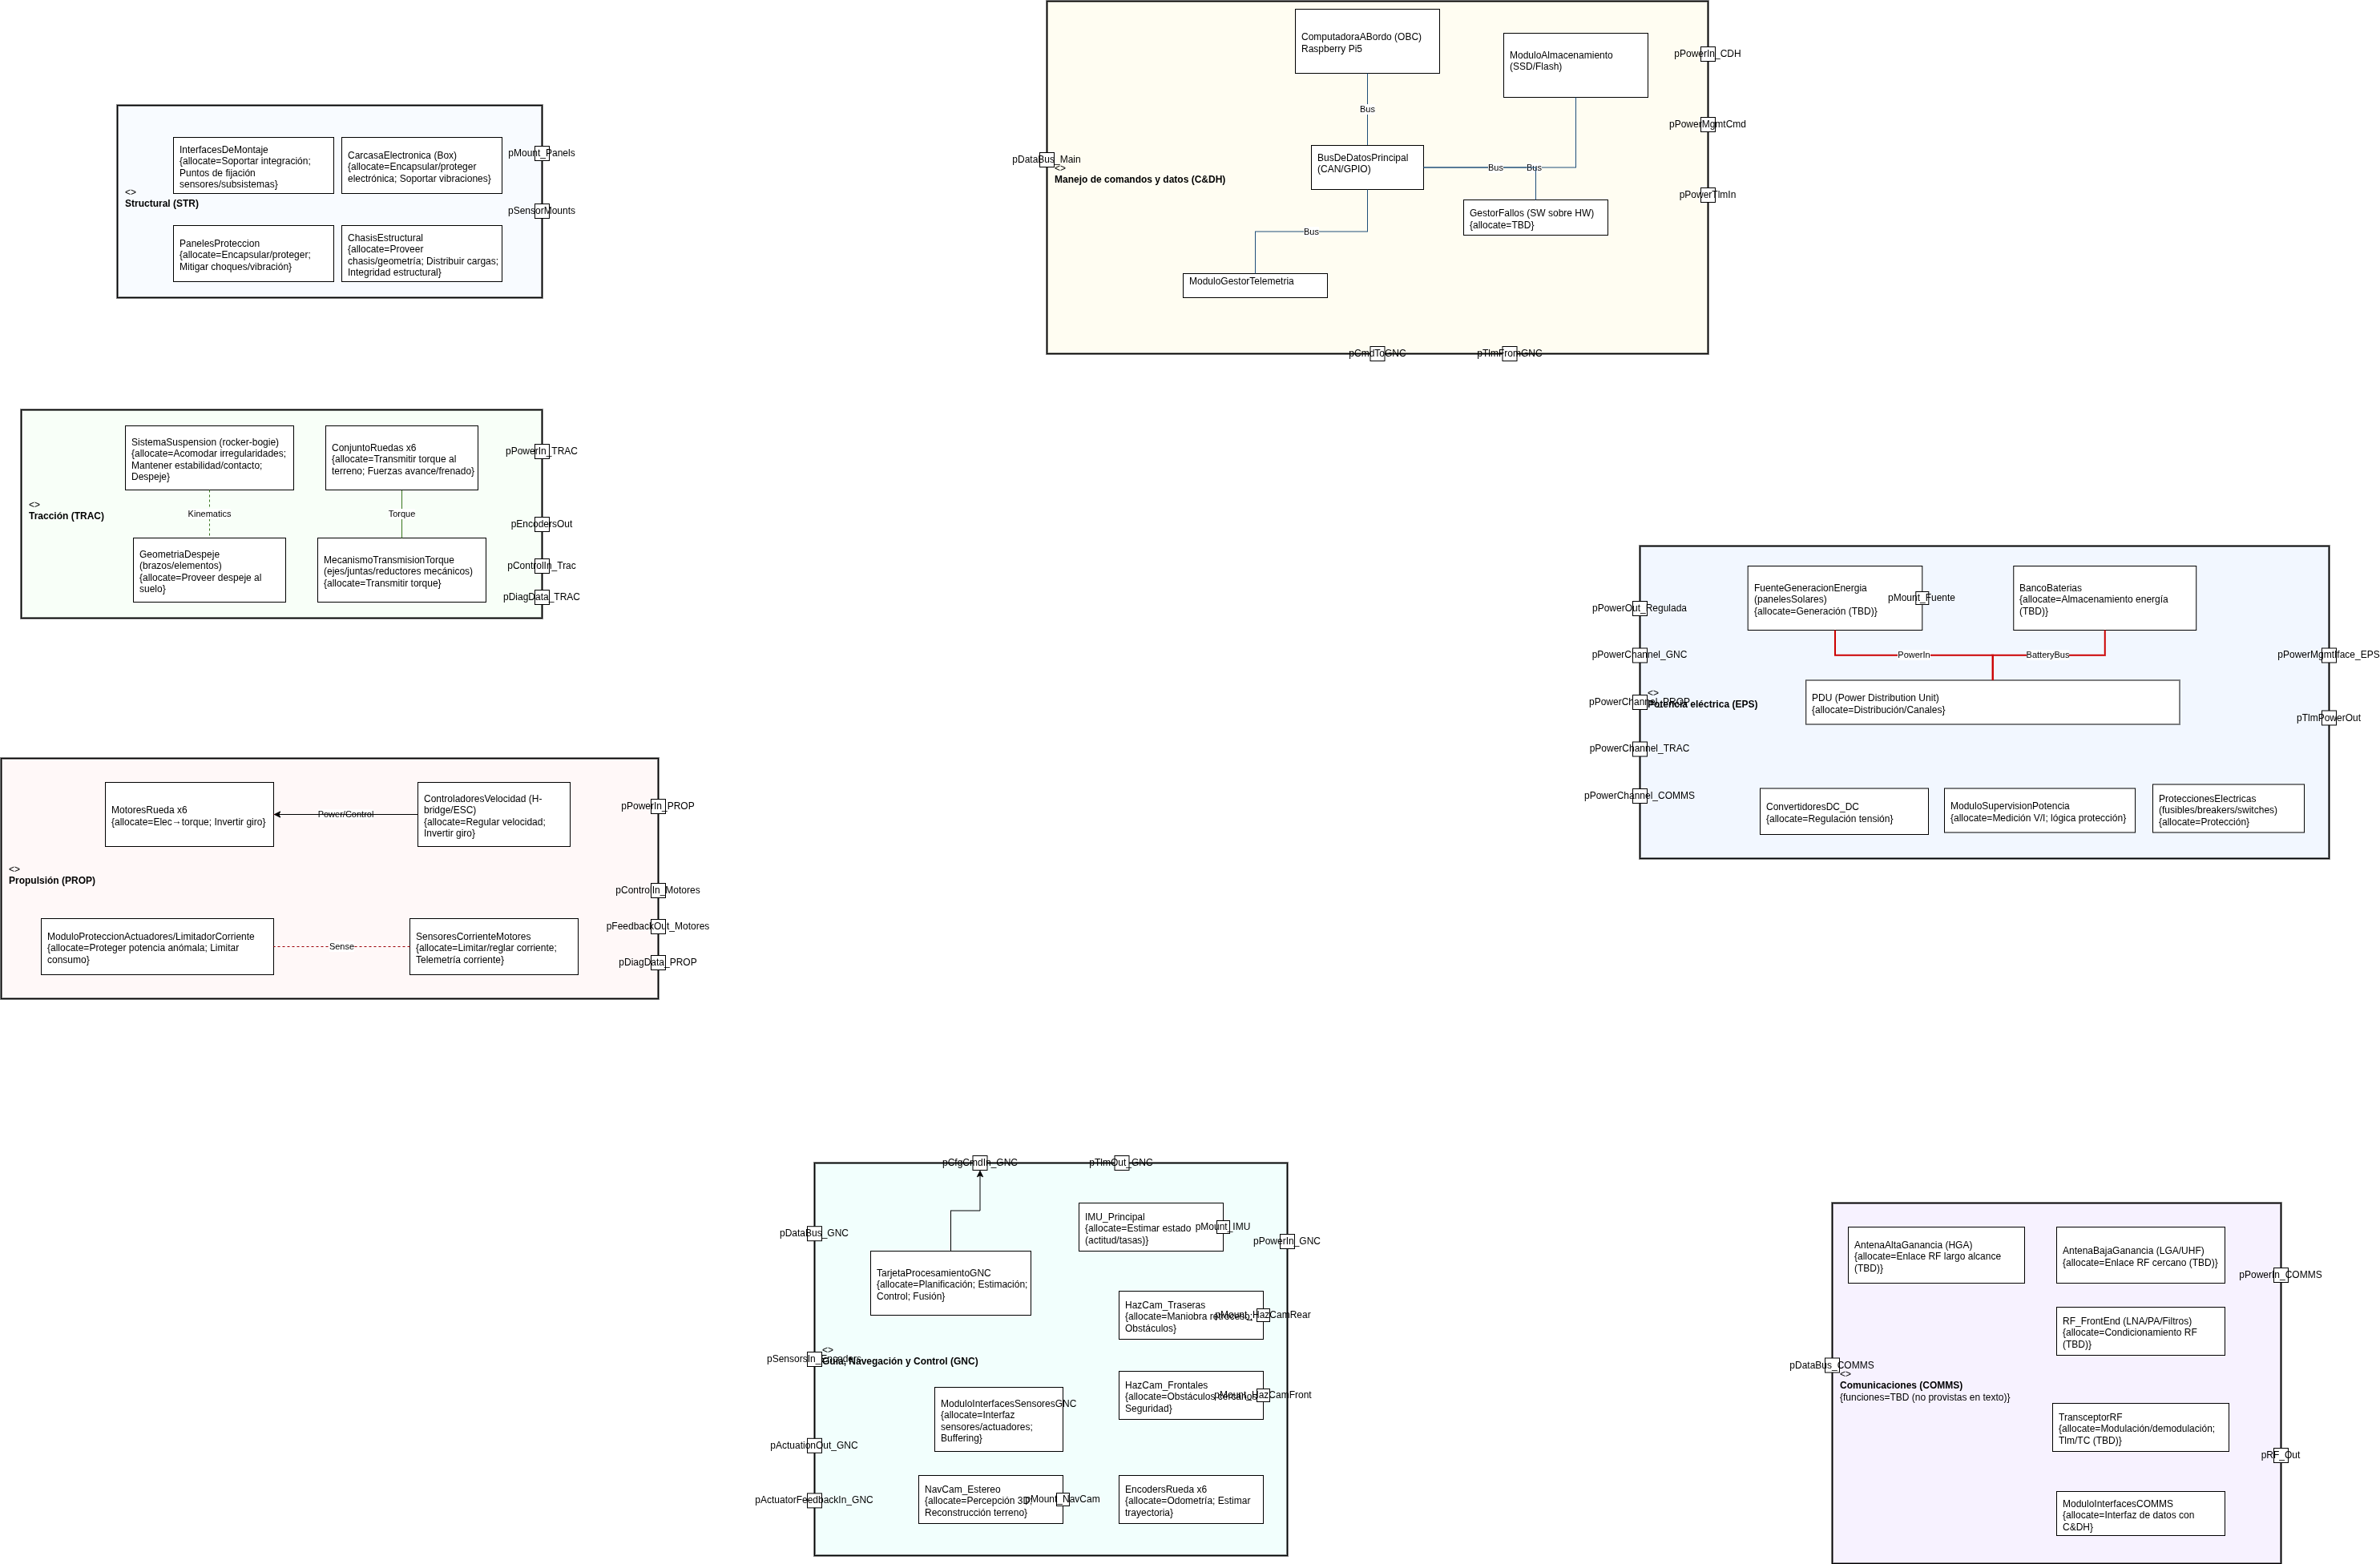
\includegraphics[width=0.95\linewidth]{figures/BDD-Page-2.drawio.png}
    \caption{Internal Block Diagram (IBD) físico del Rover Olympus: Interconexiones y puertos por subsistema.}
    \label{fig:ibd_fisico}
\end{figure}
\end{landscape}

La figura final del IBD se incluye en los anexos.

\paragraph{Subsistema de Estructura (STR)}
En primera instancia, se tiene el subsistema \textbf{Structural (STR)}, cuya responsabilidad es proveer la \textbf{base mecánica} del rover y garantizar integridad estructural durante operación. Está compuesto principalmente por \textbf{ChasisEstructural}, \textbf{CarcasaElectrónica (Avionics Box)}, \textbf{PanelesProtección} e \textbf{InterfacesDeMontaje}. 

Desde el punto de vista de interacción, STR recibe cargas externas del entorno (vibraciones, choques, cargas estáticas y dinámicas por contacto con el terreno) y las \textbf{distribuye} a través del chasis. Asimismo, STR entrega \textbf{interfaces de montaje} al resto de subsistemas: soporta y referencia físicamente sensores del GNC (p.\ ej., IMU y cámaras mediante \texttt{pSensorMounts}), aloja la electrónica de C\&DH/EPS en la bahía de aviónica, y provee puntos de fijación para la fuente de generación energética (p.\ ej., paneles) mediante \texttt{pMount\_Panels}. En el IBD, estas relaciones se modelan con conectores mecánicos tipo \textit{mount} (linea punteada), enfatizando que el intercambio es de \textbf{soporte y restricciones geométricas}, no de señales eléctricas.

\paragraph{Subsistema de Tracción (TRAC)}
El subsistema \textbf{Tracción (TRAC)} implementa el \textbf{contacto efectivo} con el terreno y la capacidad de mantener estabilidad en superficies irregulares. Sus componentes internos principales son el \textbf{SistemaSuspensión} (p.\ ej., rocker-bogie), el \textbf{ConjuntoRuedas x6}, el \textbf{MecanismoTransmisiónTorque} (ejes/juntas/reductores mecánicos) y elementos de \textbf{GeometríaDespeje}.

TRAC interactúa con el entorno a través de las ruedas: recibe reacciones del suelo (fuerzas normales, fricción, obstáculos) y, a partir del torque aplicado desde PROP, genera fuerzas de avance/frenado. Además, TRAC entrega información de movilidad a GNC mediante \textbf{EncodersRueda} y/o sensores asociados al tren de rodaje: en el IBD se representa el flujo \texttt{TRAC.pEncodersOut} $\rightarrow$ \texttt{GNC.pSensorsIn\_Encoders}. Dependiendo de la implementación final, TRAC puede incluir sensado adicional de suspensión/contacto (TBD) y exponer estados/diagnóstico al bus principal a través de C\&DH.

\paragraph{Subsistema de Propulsión (PROP)}
El subsistema \textbf{Propulsión (PROP)} convierte potencia eléctrica en \textbf{torque mecánico utilizable} para movilidad. En el modelo físico se compone de \textbf{MotoresRueda x6} (NFP-5840-31ZY-EN), \textbf{ControladoresVelocidad} con \textbf{configuración mixta} (L298N para los dos motores frontales FR/FL; BTS7960 para los cuatro motores restantes CR/CL/RR/RL, ver \texttt{rover-low-level-controller} commit \texttt{1845c4a}) y módulos de protección por canal (ACS712 por motor + INA3221 por banco).

PROP recibe energía desde EPS (canal \texttt{EPS.\allowbreak pPowerChannel\_\allowbreak PROP}\linebreak[0] $\rightarrow$ \texttt{PROP.\allowbreak pPowerIn\_PROP}) y recibe comandos de actuación desde el Arduino Mega (\texttt{MCU.\allowbreak pPWM\_Out}\linebreak[0] $\rightarrow$ \texttt{PROP.\allowbreak pControlIn\_\allowbreak Motores}). El Arduino, bajo mando de la Raspberry Pi 5, orquesta la velocidad y sentido de giro. Los eventos de diagnóstico del driver pueden reportarse localmente a la MCU para su consolidación en la telemetría del C\&DH. Esta arquitectura asegura que la ejecución del movimiento ocurra en un nodo de tiempo real, mientras que la decisión de alto nivel reside en la OBC.

\paragraph{Subsistema de Manejo de Comandos y Datos (C\&DH)}
El subsistema \textbf{C\&DH} constituye el \textbf{centro de cómputo y coordinación} del rover. En la arquitectura física se modela con una \textbf{arquitectura de dos nodos}: (i) la \textbf{Computadora a Bordo (OBC) Principal} (Raspberry Pi 5) encargada del procesamiento de IA, visión y lógica de alto nivel, y (ii) el \textbf{Nodo de Actuación} (Arduino Mega 2560 R3) especializado en la ejecución de comandos de movimiento en tiempo real. Ambos nodos se interconectan mediante un \textbf{enlace UART} dedicado.

C\&DH integra los flujos de información del sistema: la RPi 5 actúa como el \textbf{hub de percepción}, recibiendo datos directos de cámaras y sensores de rango (LiDAR/Ultrasonido), y se conecta con COMMS vía \textbf{USB (KISS)}. El Arduino Mega recibe comandos de dirección y velocidad desde la RPi 5 para gestionar los actuadores. A nivel energético, el subsistema se alimenta desde EPS (\texttt{EPS.pPowerOut\_Regulada} $\rightarrow$ \texttt{C\&DH.pPowerIn\_CDH}) y monitorea la telemetría eléctrica a través del bus I2C mediante el \textbf{INA3221} en modo bus-only (3 canales de tensión, uno por banco del EPS).

\paragraph{Subsistema de Guía, Navegación y Control (GNC)}
El subsistema \textbf{GNC} implementa la autonomía de navegación: percepción del entorno, estimación de estado y generación de comandos de movimiento. En el modelo IBD, la percepción se \textbf{distribuye en dos planos}: (i) la \textbf{Raspberry Pi 5} conecta directamente la \textbf{Cámara CSI OV5647} (pipeline YOLOv8n-seg) y el \textbf{LiDAR TF02} (UART, rango táctico para retreat); (ii) el \textbf{Arduino Mega} adquiere el \textbf{HC-SR04} ultrasonido (GPIO) y el \textbf{VL53L0X} ToF (I2C), ambos consumidos por la máquina de estados maestra (LLC) para disparar el corte de emergencia ($\le 200$\,mm en HC-SR04, $\le 150$\,mm en TF02 y $\le 50$\,mm en CLB mode). Esta distribución reduce la latencia del lazo de seguridad al evitar el cruce UART en el camino crítico de emergency-stop.

La \textbf{IMU MPU-6050} (I2C en Arduino Mega) y los \textbf{QuadratureEncoder} de rueda completan el esquema sensorial para satisfacer GNC-REQ-003, RF-004-R1 y RNF-003. GNC (ejecutado en la RPi 5) genera setpoints de movilidad que se envían vía UART al \textbf{Arduino Mega}, el cual implementa la ejecución final mediante señales **PWM** hacia los drivers de motor y servos de dirección. Se añade un canal de \emph{e-stop} cableado en EPS/PDU que garantiza la detención $\le 500$\,ms conforme a PROP-REQ-002.

GNC recibe alimentación desde EPS (\texttt{EPS.pPowerChannel\_GNC} $\rightarrow$ \texttt{GNC.pPowerIn\_GNC}). A nivel de datos, los sensores de percepción alimentan el flujo de IA en la OBC, mientras que la telemetría de navegación se consolida para su envío a COMMS. El montaje de sensores se garantiza por STR mediante puertos mecánicos (\textit{mount}), asegurando alineación y rigidez.

\paragraph{Subsistema de Comunicaciones (COMMS)}
El subsistema \textbf{COMMS} proporciona los enlaces de datos entre el rover y la estación base. En el modelo físico, se integra mediante un módulo **Wi-Fi 2.4 GHz** (nativo de la RPi 5) y un canal robusto **UHF (430-440 MHz)** basado en el NinoTNC y transceptores Kenwood. 

COMMS recibe alimentación desde EPS (\texttt{EPS.\allowbreak pPowerChannel\_\allowbreak COMMS}\linebreak[0] $\rightarrow$ \texttt{COMMS.\allowbreak pPowerIn\_\allowbreak COMMS}). La integración de datos se realiza mediante un enlace **USB (protocolo KISS)** entre la Raspberry Pi 5 y el TNC para el canal UHF, mientras que el flujo Wi-Fi se gestiona internamente en la OBC. Esto asegura que la gestión de paquetes CSP y el ruteo de telemetría se centralicen en el nodo de alto nivel del C\&DH. La interacción con el ambiente se modela mediante el puerto RF (\texttt{pRF\_Out}), incluyendo el enlace de video **FPV independiente** de 5.8 GHz.

\paragraph{Subsistema de Potencia Eléctrica (EPS)}
El subsistema \textbf{EPS} gestiona la energía del rover: almacenamiento, regulación y distribución. Sus componentes internos incluyen \textbf{3 Bancos de Baterías 18650 NMC} (rail principal + 2 rails secundarios; \textbf{sin BMS centralizado} en la arquitectura desplegada --- decisión de diseño 2026-05-17 reflejada en el driver INA3221), \textbf{Convertidores DC/DC (buck)}, \textbf{PDU} (unidad de distribución), \textbf{Protecciones Eléctricas} (fusibles por banco + relay de corte \texttt{BNK:0} accionable por GCS) y \textbf{Módulo de Supervisión de Potencia} \textbf{INA3221} (medición de tensión bus en 3 canales, modo bus-only) complementado por \textbf{ACS712} en cada motor para sensado de corriente individual y disparo de \texttt{OC\_FAULT} en el LLC. \textit{[FUTURO]} La integración de una fuente de generación fotovoltaica a bordo se contempla como trabajo futuro y no forma parte de la versión desplegada. La PDU implementa segmentación por ramas con fusibles y límites de corriente documentados en el ICD de potencia. Cada convertidor DC-DC incluirá su curva de eficiencia y su nivel de \emph{derating}. Se define una política de \emph{load-shed} para modo SAFE donde se inhabilitan secuencialmente: COMMS vídeo (FPV), GNC visión intensiva y servicios no esenciales de C\&DH.

EPS entrega potencia a los subsistemas mediante canales dedicados: \texttt{pPowerChannel\_GNC}, \texttt{pPowerChannel\_PROP}, \texttt{pPowerChannel\_TRAC} y \texttt{pPowerChannel\_COMMS}, además de una línea de \textbf{potencia regulada} hacia C\&DH (\texttt{pPowerOut\_Regulada}). En sentido de control, EPS recibe comandos de gestión de potencia desde C\&DH (\texttt{pPowerMgmtIface\_EPS}) para habilitar/inhabilitar canales o cambiar modos energéticos, y reporta telemetría de salud eléctrica (\texttt{pTlmPowerOut}) al subsistema de datos. Internamente, la \textbf{PDU} centraliza entradas desde la \textbf{Fuente} y el \textbf{BancoBaterías}, consolidando el \textit{battery bus} y distribuyendo energía hacia los convertidores/reguladores y cargas.

\paragraph{Interfaz del sistema con el ambiente (visión IBD)}
Finalmente, el IBD también permite identificar entradas externas al sistema: (i) interacción mecánica con el terreno (fuerzas en ruedas/suspensión), (ii) excitación ambiental sobre la estructura (vibración, choques, polvo/temperatura), (iii) señales ópticas del entorno capturadas por cámaras (GNC), (iv) enlace RF hacia/desde el exterior (COMMS) y (v) energía externa si existe generación (paneles) o recarga. Estas interfaces delimitan los \textbf{confines del sistema} y clarifican qué variables provienen del entorno durante operación.

\paragraph{Extensión COMMS (UHF, añadido).}
Además del enlace Wi‑Fi 2.4\,GHz, el sistema integra un canal UHF 430–440\,MHz con
modulación GFSK a 9600\,bps, empleando AX.25 (KISS) como capa de enlace y CSP como
encapsulamiento de misión. Este canal está orientado a TM/CMD robusta y habilita
operación \emph{store-and-forward} mediante un nodo retransmisor CSP cuando la LoS
directa es limitada por la topografía.

\paragraph{Selección de materiales (Construcción híbrida).}
La estructura del Rover Olympus es \textbf{híbrida}: el chasis estructural se construye con \textbf{tubería de PVC} (perfiles tubulares de la suspensión rocker-bogie heredada de POAS), acoplada mediante \textbf{piezas de manufactura aditiva} (acoples motor-eje, hubs de rueda, soportes y bahía de aviónica) y \textbf{paneles de acrílico} para la protección visible de la electrónica. Para las piezas impresas se utiliza filamento \textbf{PLA MAX}, seleccionado por su \textbf{alta tenacidad y rigidez} (densidad 1.24\,g/cm$^3$, temperatura de deformación 57\,$^{\circ}\mathrm{C}$, precisión dimensional $\pm$0.02\,mm), superando al PLA estándar en resistencia a impactos y tracción --- relevante para hubs de rueda, acoples de torque (\texttt{Acople-10}, \texttt{acople\_nfp5840\_v20}) y soportes de rodamientos F687ZZ.

% ============================================================
% 02 · HARDWARE SELECCIONADO (COTS / DEV) — ROVER OLYMPUS
% Tabla estilo "flight-qualified", adaptada a COTS académicos
% ============================================================

\subsubsection{Hardware Seleccionado (COTS / DEV)}
\label{sec:hw_selected}

Esta sección consolida los componentes físicos integrados en el Rover Olympus,
clasificados por subsistema y tipo (COTS, DEV).  
Las especificaciones y valores cuantitativos no provistos en el SyRS se
marcan como \textbf{TBD} para completarse en el ICD/BOM final.

\begin{table}[H]
\centering
\caption{Inventario de Hardware (Parte 1: C\&DH, EPS, PROP) --- Especificaciones técnicas y consumos.}
\renewcommand{\arraystretch}{1.25}
\resizebox{\textwidth}{!}{%
\begin{tabular}{p{1.9cm} p{4cm} p{3.2cm} p{4.5cm} p{1.7cm} p{1.7cm} p{1.6cm}}
\hline
\textbf{SUBSIS} &
\textbf{COMPONENTE} &
\textbf{P/N \,/\, MODELO} &
\textbf{ESPECIFICACIÓN} &
\textbf{MASA\linebreak(kg)} &
\textbf{POT.\linebreak(W)} &
\textbf{TIPO}
\\ \hline

% ---------------------
% C&DH
% ---------------------
C\&DH &
OBC Principal (Raspberry Pi 5) &
RPI 5 &
BCM2712 Quad-Core A76 @ 2.4GHz; 4GB/8GB RAM; 2x USB3.0, PCIe 2.0; MIPI CSI-2; 5V/5A (USB-C PD) &
0.046 &
2.7--12.0 &
COTS
\\
C\&DH &
Almacenamiento SSD/microSD &
\textbf{TBD} &
$\ge$ 2 h de TM/logs; interfaz USB3 &
0.050 &
1.5--4.5 &
COTS
\\
C\&DH &
MCU Arduino Mega 2560 R3 &
Mega 2560 R3 (Gen) &
ATmega2560; Nodo de actuación; Control exclusivo de Motores/Servos vía PWM &
0.037 &
0.35--1.0 &
COTS
\\

% ---------------------
% EPS
% ---------------------
EPS &
Banco de Baterías 18650 NMC (×3) &
\textbf{TBD} (LG/Samsung 18650 NMC) &
Arquitectura de 3 bancos independientes (rail principal + 2 rails secundarios); celdas Li-ion NMC 18650; capacidad y configuración serie/paralelo por banco \textbf{TBD} pendiente PDF cableado v2; \textbf{sin BMS centralizado} (balanceo externo en carga) &
\textbf{TBD} &
--- &
COTS
\\
EPS &
Monitor de tensión INA3221 &
INA3221 (Texas Instruments) &
3 canales de medición de tensión bus (uno por banco); modo bus-only (sin shunt R\_SHUNT); I2C 0x40-0x43; integrado en LLC (driver Rust 2026-05-17) &
0.002 &
< 0.001 &
COTS
\\
EPS &
Sensor de corriente ACS712 (×6) &
ACS712-30A &
Sensor Hall efecto, una unidad por motor; salida analógica 66\,mV/A; disparo \texttt{OC\_FAULT} en LLC (umbral provisional 15\,A, pendiente calibración con I\_stall NFP-5840) &
0.036 &
0.05--0.1 &
COTS
\\
EPS &
DC-DC Buck Regulados &
\textbf{TBD} &
5V/12V; conversión desde bancos $\rightarrow$ cargas internas; Eficiencia $\ge$ 85\% &
\textbf{TBD} &
\textbf{TBD} &
COTS
\\
EPS &
PDU + Fusibles por rama &
\textbf{TBD} &
Distribución y aislamiento eléctrico &
\textbf{TBD} &
\textbf{TBD} &
DEV
\\

% ---------------------
% PROPULSIÓN
% ---------------------
PROP &
Motor DC con reductora (×6) &
NFP-5840-31ZY-EN &
Worm Gear (Self-locking); 12V DC; 6 RPM; Torque nominal 70 kg$\cdot$cm; incluye encoder de efecto Hall &
0.360 &
1.0--19.2 &
COTS
\\
PROP &
Motor DC con reductora (Alt) &
JGY-370 &
Worm Gear (Self-locking); 12V DC; 40 RPM; Torque nominal 15.5 kg$\cdot$cm &
0.162 &
0.4--3.6 &
COTS
\\
PROP &
Driver Dual H-Bridge L298N (×1) &
L298N (Red) &
Dual H-Bridge; 2A cont./3A peak; $\le$ 46V DC; PWM+DIR. \textbf{Asignación}: motores frontales FR/FL únicamente (configuración mixed-drivers, LLC \texttt{1845c4a}) &
0.026 &
0.18 &
COTS
\\
PROP &
Driver High-Power BTS7960 (×4) &
BTS7960 (BTN7971) &
H-Bridge; 43A peak; 5.5--27V DC; Protecciones OC/OV/OT. \textbf{Asignación}: motores centrales y traseros CR/CL/RR/RL (configuración mixed-drivers, LLC \texttt{1845c4a}); dead-band 15\% activo &
0.264 &
0.40 &
COTS
\\
\hline
\end{tabular}}
\end{table}

\begin{table}[H]
\centering
\caption{Inventario de Hardware (Parte 2: TRAC, COMMS, GNC, STR) --- Especificaciones técnicas y consumos.}
\renewcommand{\arraystretch}{1.25}
\resizebox{\textwidth}{!}{%
\begin{tabular}{p{1.9cm} p{4cm} p{3.2cm} p{4.5cm} p{1.7cm} p{1.7cm} p{1.6cm}}
\hline
\textbf{SUBSIS} &
\textbf{COMPONENTE} &
\textbf{P/N \,/\, MODELO} &
\textbf{ESPECIFICACIÓN} &
\textbf{MASA\linebreak(kg)} &
\textbf{POT.\linebreak(W)} &
\textbf{TIPO}
\\ \hline

% ---------------------
% TRACCIÓN
% ---------------------
TRAC &
Ruedas + Hubs impresos &
\textbf{TBD} &
Filamento PLA MAX (1.75 mm); alta tenacidad y rigidez; densidad 1.24 g/cm$^3$; precisión $\pm$0.02 mm &
\textbf{TBD} &
0 &
COTS
\\
TRAC &
Rocker-Bogie simplificado &
\textbf{TBD} (heredado POAS) &
Suspensión pasiva tubular de PVC; despeje al suelo objetivo $\ge$ 10\,cm \textbf{(TBD — pendiente medición en piezas finales tras ensamblaje)} &
\textbf{TBD} &
0 &
DEV
\\
TRAC &
Servomotor de dirección &
MG996R &
Metal Gear; Torque 11 kg/cm @ 6V; 4.8--6.6V; control PWM &
0.055 &
0.06--3.0 &
COTS
\\
TRAC &
Rodamientos F687ZZ &
F687ZZ &
Bridado (Flanged); Acero; 7 mm (DI), 14 mm (DE), 5 mm (Ancho) &
0.003 &
0 &
COTS
\\

% ---------------------
% COMMS
% ---------------------
COMMS &
Wi-Fi 2.4 GHz (interfaces RPi) &
\textbf{TBD} &
Enlace UDP/IP + CSP; alcance $\ge$ 50 m (LoS) &
\textbf{TBD} &
Incl. en RPi &
COTS
\\
COMMS &
Transmisor/Receptor FPV (5.8GHz) &
AKK TS832 / RC832 &
5.8GHz 48CH; Potencia 600mW; Alcance $\ge$ 3km; Voltaje 7--16V; Conector RP-SMA. \textbf{Canal auxiliar} de monitoreo humano; no consumido por el pipeline GNC ni por el stack CSP &
0.107 &
2.6 (TX) &
COTS
\\
COMMS &
Radio UHF (Kenwood) \textbf{[FUTURO]} &
TM-D710GA/TS-2000 &
Transceptor UHF para telemetría crítica; \textbf{Alimentación Externa}. \textbf{[FUTURO]} Componente conceptual incluido para diseño extensible; \textbf{no integrado} en el stack actual --- la comunicación rover-GCS desplegada opera sobre Wi-Fi 2.4\,GHz con CSP \texttt{csp\_if\_udp} (HLC commit \texttt{3e99f8f}) &
1.500 &
Externa &
COTS
\\
COMMS &
Antenas (montaje en STR) &
\textbf{TBD} &
LGA/Omnidireccional según geometría &
\textbf{TBD} &
0 &
DEV
\\

% ---------------------
% GNC
% ---------------------
GNC &
Cámara CSI (Raspberry Pi v1.3) &
OV5647 (sensor) / RPi Cam v1.3 &
Sensor OV5647 (5 MP); video 1080p30; interfaz CSI sobre RPi5; lente \textbf{stock 54° (no 120°)} montada al 2026-05-18. \textbf{TBD}: confirmar si se reemplaza por lente M12 wide-angle ($\ge$ 120°) o se ajusta GNC-REQ-001 al FOV real &
0.003 &
1.25 &
COTS
\\
GNC &
IMU MPU-6050 &
MPU-6050 (InvenSense) &
6-DOF (giro+acelerómetro), I2C 0x68; 100--200\,Hz; conectado al Arduino Mega (LLC); INT-04b validado 2026-04-12 (responde a 0x68) &
0.005 &
0.05--0.10 &
COTS
\\
GNC &
LiDAR TF02 &
Benewake TF02 &
Rango 0.40--22\,m (acc $\pm$5\,cm); interfaz UART 115200\,bps directa a Raspberry Pi 5; integrado con fix ISR USART2 FIFO (LLC v2.17 \texttt{6dc27ec}, validado 2026-04-26 SIG=7) &
0.045 &
0.60--1.00 &
COTS
\\
GNC &
ToF VL53L0X &
VL53L0X (STMicroelectronics) &
Rango 0--2\,m (Time-of-Flight láser); interfaz I2C 0x29; conectado al Arduino Mega (LLC) en cara frontal; sensor de corte de emergencia ($\le$50\,mm en CLB mode), pendiente pull-ups validados &
0.001 &
0.02--0.04 &
COTS
\\
GNC &
Sensor Ultrasónico HC-SR04 &
HC-SR04 &
Rango 2--400\,cm; interfaz Trigger/Echo \textbf{en GPIO del Arduino Mega (LLC)} para mantener el corte de emergencia ($\le$200\,mm) fuera del camino crítico UART &
0.009 &
0.075 &
COTS
\\
GNC &
Encoders cuadratura (×6) &
Integrado NFP-5840 (Hall) &
Encoder de efecto Hall en cada motor NFP-5840-31ZY-EN (PPR \textbf{TBD} pendiente calibración \texttt{TICKS\_PER\_REV}); fase B en D44--D49; consumido por \texttt{MotorWithEncoder} en LLC v2.20 (lazo cerrado por rueda) &
--- (incl. motor) &
0.05--0.10 &
COTS
\\

% ---------------------
% STRUCTURAL
% ---------------------
STR &
Chasis tubular híbrido (PVC + 3D) &
\textbf{TBD} (heredado POAS) &
Estructura portante: \textbf{tubería de PVC} (perfiles de la suspensión rocker-bogie heredada de POAS) + \textbf{acoples e insertos impresos en PLA MAX} (alta resistencia a impactos, temp. deformación 57\,$^{\circ}$C) + paneles de acrílico para protección visible &
\textbf{TBD} &
0 &
DEV
\\
STR &
Bahía de aviónica sellada &
\textbf{TBD} &
Protección IP parcial (nivel \textbf{TBD}) &
\textbf{TBD} &
0 &
COTS
\\
STR &
Brackets para IMU/Cámara/Antenas &
\textbf{TBD} &
Alineamiento rígido; montaje preciso &
\textbf{TBD} &
0 &
DEV
\\

\hline
\end{tabular}}
\end{table}

% Nota de consistencia OS
\paragraph{Nota de consistencia de SO.}
El proyecto adopta \emph{Yocto Project} como base del sistema operativo embebido en C\&DH/GNC.
Queda desautorizada cualquier referencia previa a distribuciones genéricas (p.\,ej.\ Ubuntu).

\paragraph{COMMS UHF (componentes de integración) \textbf{[FUTURO]}.}
\textit{Esta arquitectura UHF se documenta como diseño extensible para una futura iteración del rover; no está integrada en el stack desplegado, el cual opera exclusivamente sobre Wi-Fi 2.4\,GHz con CSP (\texttt{csp\_if\_udp} nativo, HLC commit \texttt{3e99f8f}).} Diseño objetivo: TNC por hardware (\emph{NinoTNC 9600A}, KISS a 9600\,GFSK), transceptor UHF de laboratorio (\emph{Kenwood TM‑D710GA / TS‑2000}), y antenas UHF (Eggbeater para nodo móvil, Yagi para estación/retransmisor). Conexiones planeadas: C\&DH$\leftrightarrow$TNC (\textbf{USB KISS}), TNC$\leftrightarrow$Radio (audio/PTT), Radio$\leftrightarrow$Antena (RF). Alimentación desde EPS (5\,V TNC, 12\,V Radio).

% Notas de integración
\noindent\textbf{Notas.} El TNC se conecta a C\&DH por \textbf{USB} (KISS). El transceptor UHF se
interconecta por audio/datos con el TNC (incluye PTT). La potencia se suministra desde EPS
(12\,V al radio, 5\,V al TNC). La capa CSP mantiene compatibilidad con la interfaz Wi‑Fi.
La comunicación OBC$\leftrightarrow$MCU se realiza mediante \textbf{UART}.


% ============================================================
% 02.x · PRESUPUESTO DE MASA — Rover Olympus (adaptado a 7 subsistemas)
% ============================================================

\subsubsection{Presupuesto de Masa (Baseline y Márgenes)}
\label{sec:mass_budget}

Este presupuesto de masa se estructura exclusivamente según la arquitectura oficial de \textbf{7 subsistemas} del Rover Olympus —\textbf{STR}, \textbf{TRAC}, \textbf{PROP}, \textbf{C\&DH}, \textbf{EPS}, \textbf{COMMS}, \textbf{GNC}— para mantener coherencia con la vista de arquitectura ($\S$\ref{sec:architecture}) y la definición de interfaces (IBD/N2, $\S$\ref{subsec:physical_view}). Los valores no especificados en el SyRS se dejan como \textbf{TBD} y deberán cerrarse en el ICD/BOM y el reporte de integración física. \cite{nasa_cm, segoldmine_ppi}

\paragraph{Criterios.}
(a) La masa de cada subsistema es la suma de sus ítems COTS/DEV seleccionados en §\ref{sec:hw_selected}. (b) El \emph{Margen de diseño} se aplica como porcentaje sobre el subtotal (por defecto, \textbf{20\%}) mientras el proyecto esté en fase académica/integración. (c) El \emph{Límite de masa} de campaña se define a nivel de proyecto; si no existe un valor contractual, se mantiene como \textbf{TBD}. (d) Las estimaciones parciales por componente se consolidan en la PBS/N2 y el ICD de integración para evitar divergencias con el baseline de §\ref{sec:architecture}–§\ref{subsec:physical_view}. \cite{nasa_cm, segoldmine_ppi}

\begin{table}[H]
\centering
\caption{Presupuesto de masa agregado por subsistema (estimación CBE con margen AIAA del 20\%).}
\renewcommand{\arraystretch}{1.20}
\begin{tabular}{p{7.5cm} r}
\hline
\textbf{Bloque / Rubro} & \textbf{Masa [kg]} \\
\hline
\textbf{STR — Estructura / Chasis híbrido (PVC + 3D + acrílico)} & 2.700 \\
\textit{(Tubería PVC heredada POAS + acoples impresos PLA MAX + bahía de aviónica + brackets/mounts)} & \\[1ex]

\textbf{TRAC — Tracción (Locomotion)} & 1.591 \\
\textit{(Ruedas + hubs, rodamientos F687ZZ, servomotor de dirección MG996R)} & \\[1ex]

\textbf{PROP — Propulsión (Drive / Actuación)} & 2.550 \\
\textit{(Motores NFP-5840-31ZY-EN ×6, drivers mixtos L298N×1 + BTS7960×4, acoples)} & \\[1ex]

\textbf{C\&DH — Command \& Data Handling} & 0.183 \\
\textit{(RPi 5 única, MCU Arduino Mega, SSD/microSD, cableado)} & \\[1ex]

\textbf{EPS — Energía (3 bancos + DC/DC + PDU)} & 0.638 \\
\textit{(3 bancos 18650 NMC, sin BMS centralizado, INA3221 monitor V, ACS712 ×6 sensado I, convertidores DC/DC, PDU)} & \\[1ex]

\textbf{COMMS — Comunicaciones} & 0.197 \\
\textit{(Wi-Fi 2.4\,GHz nativo RPi5, FPV TS832/RC832 auxiliar, antenas; UHF [FUTURO] no contabilizado)} & \\[1ex]

\textbf{GNC — Guía, Navegación y Control} & 0.146 \\
\textit{(Cámara OV5647, IMU MPU-6050, LiDAR TF02, ToF VL53L0X, HC-SR04, encoders Hall integrados en motores)} & \\[1ex]

\textbf{MISC — Otros (Tornillería, cables, adhesivos)} & 0.500 \\
\hline
\textbf{SUBTOTAL (sin margen)} & 8.505 \\
\textbf{Margen de diseño (20\% del subtotal)} & 1.701 \\
\hline
\textbf{MASA TOTAL (con margen)} & \textbf{10.206} \\
\hline
\textbf{LÍMITE DE MASA (campaña / proyecto)} & \textbf{10.500} \\
\textbf{MARGEN vs. LÍMITE} & \textbf{+0.294} \\
\hline
\end{tabular}
\end{table}

\paragraph{Notas y plan de cierre.}
\begin{itemize}
  \item \textbf{Fuentes de masa por ítem}: tabla de hardware de §\ref{sec:hw_selected} y BOM del PBS; consolidar en ICD con evidencia (fichas técnicas, pesaje de banco). \cite{nasa_cm}
  \item \textbf{Criterio de margen}: 20\% mientras existan \textbf{TBD} significativos en componentes/impresiones; ajustar a un margen por subsistema cuando el diseño esté congelado y existan pesajes reales. \cite{nasa_cm, segoldmine_ppi}
  \item \textbf{Consistencia con N2/IBD}: verificar que toda adición mecánica (brackets, herrajes, cableado con masa relevante) esté asignada al subsistema correcto para evitar \emph{underestimation}. \cite{nasa_cm}
\end{itemize}

\paragraph{Placeholders para completar (ICD/BOM).}
\begin{enumerate}
  \item Masa por componente COTS/DEV (STR, TRAC, PROP, C\&DH, EPS, COMMS, GNC): \textbf{Completado (CBE)}.
  \item Subtotal por subsistema y \% de contribución al total: \textbf{Definido en Tabla 10.2.x}.
  \item Límite de masa de campaña (si aplica al sitio análogo): \textbf{10.500 kg}.
\end{enumerate}
% ============================================================
% 02.y · PRESUPUESTO DE POTENCIA — Rover Olympus (7 subsistemas)
% ============================================================

\subsubsection{Presupuesto de Potencia (Modos Operacionales)}
\label{sec:power_budget}

Este presupuesto se organiza estrictamente por los \textbf{7 subsistemas} del Rover Olympus —\textbf{STR}, \textbf{TRAC}, \textbf{PROP}, \textbf{C\&DH}, \textbf{EPS}, \textbf{COMMS}, \textbf{GNC}— y por \emph{modos} coherentes con el ConOps y la máquina de estados: \textbf{SCIENCE / Exploración activa}, \textbf{CRUISE / Tránsito nominal}, \textbf{SAFE / Modo seguro}. Los valores se consolidarán a partir de la tabla de hardware ($\S$\ref{sec:hw_selected}) y de las especificaciones de integración definidas en la arquitectura física (IBD) y la matriz N2 ($\S$\ref{sec:architecture}--$\S$\ref{subsec:physical_view}). \textit{En este proyecto académico (lab-only) no existe generación continua a bordo (p.\,ej., paneles); la energía proviene del banco de baterías EPS, por lo que el presupuesto refleja \emph{consumo} y \emph{autonomía} esperada, no balance GEN--LOAD.} \cite{nasa_cm}

\paragraph{Criterios y supuestos.}
(a) \textbf{SCIENCE} corresponde al modo \emph{Exploración activa} (carga de sensado/visión, planificación y comando de actuadores). (b) \textbf{CRUISE} es un tránsito nominal con percepción y comunicaciones en carga reducida. (c) \textbf{SAFE} minimiza cargas (COMMS esenciales, C\&DH básico) para preservar integridad. (d) Los valores no definidos en el SyRS se marcan \textbf{TBD} y deberán cerrarse en el ICD de EPS (niveles de tensión/corriente, distribución por ramas) y en el BOM/PBS. (e) La asignación de buses y líneas de potencia se rige por el IBD/N2 físico del sistema. \cite{nasa_cm}

% -------------------------------
% Tabla por subsistema y modo
% -------------------------------
\begin{table}[H]
\centering
\caption{Presupuesto de potencia por subsistema: Consumo nominal basado en componentes COTS integrados.}
\renewcommand{\arraystretch}{1.20}
\resizebox{\textwidth}{!}{%
\begin{tabular}{p{5.5cm} r r r p{5.5cm}}
\hline
\multirow{2}{*}{\textbf{Subsistema / Carga}} & \multicolumn{3}{c}{\textbf{Potencia \,[W] por Modo}} & \multirow{2}{*}{\textbf{Notas}} \\
\cline{2-4}
 & \textbf{SCIENCE} & \textbf{CRUISE} & \textbf{SAFE} & \\
\hline
\textbf{GNC} (RPi5 + OV5647 + TF02 + VL53L0X + MPU-6050 + HC-SR04) & 14.50 & 5.50 & 0.50 & Percepción YOLOv8n-seg + rango táctico activo. \\
\textbf{C\&DH} (RPi5 OBC única + Arduino Mega + SSD/microSD) & 7.00 & 3.00 & 2.00 & Orquestación y ruteo de datos; sin RPi4 auxiliar (single-node). \\
\textbf{PROP} (Motores NFP-5840 ×6 + drivers mixtos L298N+BTS7960) & 115.20 & 38.40 & 0.00 & Rating nominal 1.6A/motor @ 12V; dead-band 15\% activo. \\
\textbf{TRAC} (Servomotor MG996R) & 3.00 & 1.00 & 0.00 & Dirección activa en exploración. \\
\textbf{COMMS} (Wi-Fi 2.4\,GHz nativo RPi5 + FPV TS832 auxiliar) & 2.60 & 0.50 & 0.50 & UHF [FUTURO] no contabilizado; CSP \texttt{csp\_if\_udp} sobre WiFi. \\
\textbf{EPS} (Pérdidas DC/DC + INA3221 + ACS712 ×6) & 21.10 & 7.10 & 0.40 & Eficiencia calculada del 85\%; sin BMS centralizado. \\
\textbf{STR} (pasivo) & 0 & 0 & 0 & Estructura pasiva. \\
\hline
\textbf{TOTAL por modo} & \textbf{163.40} & \textbf{55.50} & \textbf{3.40} &  \\
\hline
\end{tabular}}
\end{table}

% -------------------------------
% Tabla de modos agregados y margen
% -------------------------------
\begin{table}[H]
\centering
\caption{Potencia agregada por modo y margen de diseño conservador del 20\%.}
\renewcommand{\arraystretch}{1.20}
\begin{tabular}{p{7.5cm} r}
\hline
\textbf{Modo Operacional} & \textbf{Potencia Total \,[W]} \\
\hline
\textbf{SCIENCE (Exploración activa)} & 163.40 \\
\textbf{CRUISE (Tránsito nominal)} & 55.50 \\
\textbf{SAFE (Modo seguro)} & 3.40 \\
\hline
\textbf{Consumo pico considerado (SCIENCE)} & 163.40 \\
\textbf{Margen de diseño (energía), 20\% sobre pico} & 32.68 \\
\hline
\end{tabular}
\end{table}

\paragraph{Análisis de Autonomía (3 bancos 18650 NMC --- capacidad total \textbf{TBD}).}
La arquitectura EPS desplegada (decisión de diseño 2026-05-17) emplea 3 bancos independientes de celdas 18650 NMC sin BMS centralizado; la capacidad total por banco y la configuración serie/paralelo quedan \textbf{TBD} pendiente PDF cableado v2. Las estimaciones de autonomía previas (basadas en pack 4S2P LG MJ1 = 101.78\,Wh) deben recalcularse una vez consolidada la nueva arquitectura. Como referencia provisional, asumiendo capacidad agregada equivalente ($\sim$100\,Wh) y los nuevos consumos por modo:
\begin{itemize}
    \item \textbf{Modo SCIENCE:} $\sim$37 minutos (100\,Wh / 163.4\,W; operación continua de 6 motores a torque nominal).
    \item \textbf{Modo CRUISE:} $\sim$1.8 horas (100\,Wh / 55.5\,W; desplazamiento nominal y telemetría).
    \item \textbf{Modo SAFE:} $\sim$29.4 horas (100\,Wh / 3.4\,W; supervivencia y monitoreo de enlace).
\end{itemize}
Estas cifras se reemplazarán por medidas reales tras consolidación de la BOM EPS (capacidad real por banco) y registro de telemetría INA3221 + ACS712 en campañas. La integración UHF queda \textbf{[FUTURO]} y no afecta el perfil de autonomía actual.

\paragraph{Notas de integración (por cerrar en ICD/BOM).}
\begin{itemize}
  \item \textbf{Distribución EPS}: documentar eficiencias de cada convertidor DC/DC (rail 5\,V/12\,V), pérdidas en PDU y criterio de \emph{derating}; capturar en ICD con pruebas de banco. \cite{nasa_cm}
  \item \textbf{Perfiles de carga por modo}: instrumentar telemetría de tensión bus con INA3221 (3 canales, modo bus-only) y de corriente por motor con ACS712 (Hall, 6 unidades) en campañas; registrar series para estimar \emph{typical}/\emph{peak} por subsistema y alimentar esta tabla y el análisis de autonomía. \cite{nasa_cm}
  \item \textbf{Cargas pico de PROP}: establecer casos límite (arranque en pendiente, evitación reactiva, Fault Stop) y medir demanda dinámica para validar requisitos de movilidad y tiempos de paro. \cite{nasa_cm}
  \item \textbf{COMMS}: definir perfiles de transmisión (duty-cycle TM/CMD, vídeo FPV opcional) y su impacto por modo (SCIENCE/CRUISE/SAFE). \cite{nasa_cm}
\end{itemize}

\paragraph{Resumen.}
Este presupuesto de potencia es consistente con la arquitectura física (IBD/N2) y con los modos operacionales definidos para UC-01; al cerrarse los \textbf{TBD} con medidas reales de banco/campaña, la tabla pasará a ser el insumo directo para: (i) la verificación de \emph{autonomía} (capacidad del pack 4S vs perfiles de carga), (ii) el dimensionamiento final de convertidores/reglas de derating y (iii) la validación de contingencias (SAFE/HomingRetreat) conforme a $\S$\ref{sec:hw_selected}--$\S$\ref{subsec:software_functional_view}. \cite{nasa_cm}

% ============================================================
% 08.x · PHYSICAL BREAKDOWN STRUCTURE (PBS) + ASM Registry
% Rover Olympus — Alineado a la arquitectura de 7 subsistemas
% ============================================================

\subsubsection{Physical Breakdown Structure (PBS) y Registro ASM}
\label{sec:pbs_asm}

Esta sección define la \textbf{Estructura de Descomposición Física (PBS)} del \emph{Rover Olympus} y el \textbf{registro de identificadores de ensamble (ASM-xxxx)} para trazabilidad física. La jerarquía PBS se alinea estrictamente con los \textbf{7 subsistemas} del baseline: \textbf{STR}, \textbf{TRAC}, \textbf{PROP}, \textbf{C\&DH}, \textbf{EPS}, \textbf{COMMS}, \textbf{GNC}. Las descripciones y ejemplos de componentes se derivan de $\S$\ref{sec:architecture} (vista funcional/física, PBS reducido) y $\S$\ref{subsec:physical_view} (N2/IBD). \textit{Ningún subsistema fuera de estos 7 es introducido.} \cite{nasa_cm, segoldmine_ppi}

% ------------------------------------------------------------
% A. Jerarquía PBS (L0 → L3)
% ------------------------------------------------------------
\paragraph{Jerarquía PBS (L0$\rightarrow$L3).}
\label{subsec:pbs_hierarchy}

\noindent\textbf{PBS--L0 (Sistema)} \cite{nasa_cm}
\begin{itemize}
  \item \textbf{PBS--L0.1} \; \textit{Rover\_Olympus} (Sistema) --- límite físico del sistema en $\S$\ref{subsec:physical_view}; arquitectura en $\S$\ref{sec:architecture}; I/F externas $\S$\ref{sec:architecture}.
\end{itemize}

\noindent\textbf{PBS--L1 (Subsistemas --- 7 bloques)} \emph{(composición del sistema; ver BDD $\S$\ref{sec:architecture})} \cite{nasa_cm}
\begin{itemize}
  \item \textbf{STR} Structural (chasis tubular PVC heredado POAS + acoples impresos PLA MAX, bahía aviónica, paneles acrílicos, \emph{mounts}).
  \item \textbf{TRAC} Tracción (ruedas, hubs impresos PLA MAX, suspensión rocker-bogie pasiva, rodamientos F687ZZ).
  \item \textbf{PROP} Propulsión (motores DC NFP-5840-31ZY-EN ×6, drivers mixtos L298N×1 + BTS7960×4, acoples motor-eje, disipación).
  \item \textbf{C\&DH} Command \& Data Handling (RPi5 OBC única, MCU Arduino Mega 2560 R3, almacenamiento SSD/microSD, bus de datos UART/I2C/USB).
  \item \textbf{EPS} Energía (3 bancos 18650 NMC sin BMS centralizado, INA3221 monitor V bus, ACS712 ×6 sensado I por motor, DC/DC, PDU/fusibles, relay e-stop \texttt{BNK:0}).
  \item \textbf{COMMS} Comunicaciones (Wi‑Fi 2.4\,GHz nativo RPi5 con CSP \texttt{csp\_if\_udp}, FPV TS832/RC832 auxiliar, antenas y \emph{mounts}; UHF [FUTURO] no integrado).
  \item \textbf{GNC} Guía, Navegación y Control (cámara CSI OV5647, IMU MPU-6050, LiDAR TF02, ToF VL53L0X, HC-SR04 en Arduino Mega, encoders Hall integrados NFP-5840).
\end{itemize}

\noindent\textbf{PBS--L2 (Ensamblajes por subsistema)} \emph{(ejemplos representativos; ver $\S$\ref{sec:architecture})} \cite{nasa_cm}
\begin{itemize}
  \item \textbf{STR}: Chasis tubular PVC + acoples 3D; Bahía de aviónica; Placas de refuerzo; Brackets de sensores/antenas.
  \item \textbf{TRAC}: Conjunto rueda+hub ($\times$6); Conjunto suspensión pasiva (rocker-bogie heredada POAS).
  \item \textbf{PROP}: Conjunto motor+reductora ($\times$6, NFP-5840); Conjunto driver L298N (×1, FR/FL); Conjunto driver BTS7960 (×4, CR/CL/RR/RL); Conjunto disipación.
  \item \textbf{C\&DH}: OBC principal (RPi5, única); MCU I/O (Arduino Mega 2560 R3); Módulo de almacenamiento (microSD/SSD); Segmento del bus de datos.
  \item \textbf{EPS}: 3 Bancos 18650 NMC; Monitor de tensión INA3221 (I2C, 3 canales); Sensor de corriente ACS712 (×6, Hall); Conjunto DC/DC 5/12V; PDU+fusibles+relay \texttt{BNK:0}.
  \item \textbf{COMMS}: NIC Wi‑Fi 2.4\,GHz (nativo RPi5); FPV TX/RX (auxiliar humano); Antenas + \emph{mounts}; \textbf{[FUTURO]}: TNC NinoTNC, transceptor UHF, antenas UHF.
  \item \textbf{GNC}: Cámara CSI OV5647 (sensor v1.3); IMU MPU-6050 (I2C); LiDAR TF02 (UART); ToF VL53L0X (I2C); Sensor HC-SR04 (GPIO Arduino Mega); Encoders Hall NFP-5840 ($\times$6).
\end{itemize}

\noindent\textbf{PBS--L3 (Componentes/ítems COTS/DEV)} \emph{(detalles cerrados en BOM/ICD; ver $\S$\ref{sec:hw_selected} y $\S$\ref{subsec:physical_view})} \cite{nasa_cm}
\begin{itemize}
  \item Ej.: Rodamientos F687ZZ; cables/conectores por bus; tornillería/inserciones; sensores específicos; tarjeta INA3221; tarjetas ACS712 (×6); etc. \emph{(P/N y masa/potencia $\rightarrow$ BOM; pines/buses/voltajes $\rightarrow$ ICD)}.
\end{itemize}

% ------------------------------------------------------------
% B. Registro ASM (identificadores de ensamble — sample baseline)
% ------------------------------------------------------------
\paragraph{Registro de Identificadores de Ensamble (ASM).}
\label{subsec:asm_registry}

Los siguientes \textbf{ASM-ids} se asignan para habilitar trazabilidad \emph{PBS $\leftrightarrow$ N2/IBD $\leftrightarrow$ ICD/BOM} y soportar V\&V y control de configuración. La columna \emph{Interfaces clave} referencia el Cuadro N2/$\S$\ref{subsec:physical_view} (p.\,ej., \texttt{[PWR]}, \texttt{[DATA]}, \texttt{[CTRL]}, \texttt{[MEC]}). Los campos no definidos en el SyRS quedan \textbf{TBD}. \cite{nasa_cm}

\begin{table}[H]
\centering
\caption{Registro ASM (Parte 1: STR, TRAC, PROP, C\&DH) --- Identificadores de ensamble por subsistema.}
\renewcommand{\arraystretch}{1.15}
\resizebox{\textwidth}{!}{%
\begin{tabular}{p{1.8cm} p{1.2cm} p{1.6cm} p{4.5cm} p{5.0cm} p{1.3cm} p{2.5cm}}
\hline
\textbf{ASM-ID} & \textbf{PBS} & \textbf{Subsys} & \textbf{Ensamble / Ítem} & \textbf{Interfaces clave (N2)} & \textbf{Tipo} & \textbf{P/N} \\
\hline
ASM-010 & L2 & STR & Chasis estructural (marco + refuerzos) & [MEC] soporte TRAC/\allowbreak PROP/\allowbreak C\&DH/\allowbreak EPS/\allowbreak COMMS/\allowbreak GNC & COTS & \textbf{TBD} \\
ASM-011 & L2 & STR & Bahía de aviónica (envolvente) & [MEC] mounts; nivel IP \textbf{TBD} & COTS & \textbf{TBD} \\
ASM-012 & L3 & STR & Brackets/mounts sensores/antenas & [MEC] alineación IMU/cámara/antenas & DEV & \textbf{TBD} \\

ASM-020 & L2 & TRAC & Conjunto rueda+hub \#1 & [MEC] acople PROP; [DATA] enc.$\rightarrow$GNC & COTS & \textbf{TBD} \\
ASM-021 & L2 & TRAC & Conjunto rueda+hub \#N & [MEC] idem; [DATA] opcional & COTS & \textbf{TBD} \\
ASM-022 & L2 & TRAC & Suspensión pasiva (rocker/bogie) & [MEC] contacto terreno/estabilidad & DEV & \textbf{TBD} \\
ASM-024 & L3 & TRAC & Servomotor de dirección (MG996R) & [MEC] giro; [CTRL] PWM$\rightarrow$MCU & COTS & MG996R \\
ASM-023 & L3 & TRAC & Rodamientos F687ZZ & [MEC] soporte ejes & COTS & F687ZZ \\

ASM-030 & L2 & PROP & Motor+reductora \#1 & [PWR] EPS$\rightarrow$PROP; [CTRL] GNC/\allowbreak MCU$\rightarrow$driver; [MEC] TRAC & COTS & NFP-5840-31ZY-EN \\
ASM-030b & L2 & PROP & Motor+reductora (Alt) & [PWR]/[CTRL]/[MEC] & COTS & JGY-370 \\
ASM-031 & L2 & PROP & Motor+reductora \#N & [PWR]/[CTRL]/[MEC] & COTS & NFP-5840-31ZY-EN \\
ASM-032 & L2 & PROP & Driver motor (L298N) \textbf{×1}, FR/FL & [PWR] EPS; [CTRL] PWM+DIR; [DATA] diag$\rightarrow$C\&DH & COTS & L298N (Red) \\
ASM-032b & L2 & PROP & Driver High-Power (BTS7960) \textbf{×4}, CR/CL/RR/RL & Driver primario alta corriente (43A); [PWR]/[CTRL]/[DATA]; config mixed-drivers LLC \texttt{1845c4a} & COTS & BTS7960 \\
ASM-033 & L3 & PROP & Disipación/soportes drivers & [MEC]/térmico & DEV & \textbf{TBD} \\

ASM-040 & L2 & C\&DH & OBC única (Raspberry Pi 5) & [PWR] EPS 5V; [DATA] bus principal; [DATA] CSI; single-node sin redundancia & COTS & RPI 5 \\
ASM-042 & L2 & C\&DH & MCU Arduino Mega 2560 R3 & [PWR]; [CTRL] Motores/Servos (PWM); [DATA] I2C sensores LLC & COTS & Mega 2560 R3 \\
ASM-043 & L3 & C\&DH & Almacenamiento SSD/microSD & [DATA] USB/SD; [PWR] 5V & COTS & \textbf{TBD} \\
ASM-044 & L3 & C\&DH & Interfaces USB / UART & [DATA] Enlaces USB (TNC) y UART (MCU) & DEV & \textbf{TBD} \\
\hline
\end{tabular}}
\end{table}

\begin{table}[H]
\centering
\caption{Registro ASM (Parte 2: EPS, COMMS, GNC) --- Identificadores de ensamble por subsistema.}
\renewcommand{\arraystretch}{1.15}
\resizebox{\textwidth}{!}{%
\begin{tabular}{p{1.8cm} p{1.2cm} p{1.6cm} p{4.5cm} p{5.0cm} p{1.3cm} p{2.5cm}}
\hline
\textbf{ASM-ID} & \textbf{PBS} & \textbf{Subsys} & \textbf{Ensamble / Ítem} & \textbf{Interfaces clave (N2)} & \textbf{Tipo} & \textbf{P/N} \\
\hline
ASM-050 & L2 & EPS & 3 Bancos Li-ion 18650 NMC & [PWR] rail principal + 2 secundarios; capacidad/configuración por banco \textbf{TBD}; sin BMS centralizado & COTS & \textbf{TBD} \\
ASM-052 & L2 & EPS & Convertidores DC/DC 5/12V & [PWR] regulación; eficiencias \textbf{TBD} & COTS & \textbf{TBD} \\
ASM-053 & L2 & EPS & PDU + fusibles + relay \texttt{BNK:0} & [PWR] segmentación/aislamiento; e-stop accionable por GCS (ICD-LLC-001) & DEV & \textbf{TBD} \\
ASM-054 & L3 & EPS & INA3221 (monitor V bus, 3 canales) & [HK] telemetría EPS$\rightarrow$LLC (I2C, modo bus-only) & COTS & INA3221 \\
ASM-055 & L3 & EPS & Sensores ACS712 ($\times$6, Hall) & [HK] sensado I por motor (66\,mV/A); [CTRL] disparo \texttt{OC\_FAULT} en LLC & COTS & ACS712-30A \\

ASM-060 & L2 & COMMS & NIC Wi‑Fi 2.4\,GHz nativo RPi5 & [DATA] UDP/IP + CSP \texttt{csp\_if\_udp}; [PWR] incl. RPi5; enlace primario rover-GCS desplegado & COTS & incl. RPi5 \\
ASM-061 & L2 & COMMS & Transmisor/Receptor FPV (5.8GHz) & [DATA] vídeo auxiliar humano (no consumido por GNC); [PWR] 7--16V & COTS & TS832 / RC832 \\
ASM-062 & L3 & COMMS & Antenas + mounts & [MEC]; [RF] enlace externo & DEV & \textbf{TBD} \\

% --- Ensambles COMMS (UHF) [FUTURO] — no integrados en stack actual ---
ASM-063 & L2 & COMMS & \textbf{[FUTURO]} TNC NinoTNC 9600A & \textbf{[FUTURO]} No integrado en stack actual; [DATA] USB/UART (KISS) C\&DH$\leftrightarrow$TNC; [CTRL] PTT; [PWR] 5V & COTS & \textbf{TBD} \\
ASM-064 & L2 & COMMS & \textbf{[FUTURO]} Transceptor UHF (TM-D710GA/TS-2000) & \textbf{[FUTURO]} No integrado; [AUDIO/DATA] TNC$\leftrightarrow$Radio; [RF] Radio$\leftrightarrow$Antena; [PWR] 12V & COTS & \textbf{TBD} \\
ASM-065 & L3 & COMMS & \textbf{[FUTURO]} Antenas UHF (Eggbeater/Yagi) + coax & \textbf{[FUTURO]} No integradas; [RF] Radio$\leftrightarrow$Antena; [MEC] montaje en STR & COTS & \textbf{TBD} \\

ASM-070 & L2 & GNC & Cámara CSI OV5647 (NavCam) & [DATA] CSI; [MEC] alineación óptica; lente stock 54° (TBD: M12 wide-angle 120°) & COTS & OV5647 (RPi Cam v1.3) \\
ASM-071 & L2 & GNC & IMU MPU-6050 (6-DOF) & [DATA] I2C 0x68 (Arduino Mega); [MEC] orientación; 100--200\,Hz & COTS & MPU-6050 \\
ASM-072 & L2 & GNC & LiDAR TF02 (Rango 0.40--22\,m) & [DATA] UART 115200 $\rightarrow$ RPi 5; [PWR] 5V; ISR FIFO fix LLC v2.17 \texttt{6dc27ec} & COTS & Benewake TF02 \\
ASM-073 & L3 & GNC & Encoders Hall integrados ($\times$6) & [DATA] cuadratura phase A/B en D44--D49; integrados NFP-5840; \texttt{MotorWithEncoder} LLC v2.20 & COTS & incl. NFP-5840 \\
ASM-074 & L3 & GNC & Sensor HC-SR04 (Ultrasónico) & [DATA/CTRL] Trigger/Echo $\rightarrow$ \textbf{Arduino Mega} (GPIO LLC); corte emergencia $\le$200\,mm & COTS & HC-SR04 \\
ASM-075 & L3 & GNC & ToF VL53L0X (láser) & [DATA] I2C 0x29 $\rightarrow$ Arduino Mega; rango 0--2\,m; corte emergencia CLB $\le$50\,mm; pull-ups pendientes & COTS & VL53L0X \\
\hline
\end{tabular}}
\end{table}

% ------------------------------------------------------------
% C. Reglas de numeración, trazabilidad y cierre (ICD/BOM)
% ------------------------------------------------------------
\paragraph{Reglas de numeración y cierres (ICD/BOM).}
\label{subsec:asm_rules}

\begin{enumerate}
  \item \textbf{Bloques de numeración:} reservar rangos por subsistema (\texttt{ASM-01x}=STR, \texttt{02x}=TRAC, \texttt{03x}=PROP, \texttt{04x}=C\&DH, \texttt{05x}=EPS, \texttt{06x}=COMMS, \texttt{07x}=GNC) para facilitar lectura. \cite{nasa_cm}
  \item \textbf{Nivel PBS:} anotar \texttt{PBS=L2/L3} para distinguir ensamble vs. componente. La revisión cambia cuando varía forma/ajuste/función. \cite{nasa_cm}
  \item \textbf{Trazabilidad cruzada:} cada \texttt{ASM-xx} debe enlazar a: (i) fila de BOM (P/N, masa, potencia), (ii) entradas N2/IBD (interfaces \texttt{[PWR/DATA/CTRL/MEC/HK]}), (iii) requisitos asociados (RF/RNF/CON) y (iv) procedimientos V\&V. \cite{nasa_cm}
  \item \textbf{Cierre en ICD/BOM:} completar \textbf{P/N}, masa/potencia por ítem y conectores/pines/buses de cada interfaz antes de \emph{freeze} de integración. \cite{nasa_cm}
\end{enumerate}

\paragraph{Notas.}
(i) Los \emph{placeholders} \textbf{TBD} se cierran con mediciones de banco y con definición de conectividad (ICD); (ii) el N2 de $\S$\ref{subsec:physical_view} resume las rutas por tipo \texttt{[MEC/PWR/CTRL/DATA/HK]}; (iii) la lista ASM aquí presentada es una \emph{línea base} inicial y puede refinarse durante I\&T respetando los rangos. \cite{nasa_cm}

% ============================================================
% 08.x · BILL OF MATERIALS (BOM) — Rover Olympus
% Alineado con PBS/ASM y la arquitectura de 7 subsistemas
% Fuente base: SyRS main.pdf (§8 Arquitectura; §9 Interfaces; PBS/N2)
% ============================================================

\subsubsection{Bill of Materials (BOM)}
\label{sec:bom}

Este \textbf{BOM} consolida los ítems físicos del \emph{Rover Olympus} y mantiene trazabilidad directa con el \textbf{PBS/ASM} (véase $\S$\ref{sec:pbs_asm}) y con la arquitectura de \textbf{7 subsistemas} (\textbf{STR}, \textbf{TRAC}, \textbf{PROP}, \textbf{C\&DH}, \textbf{EPS}, \textbf{COMMS}, \textbf{GNC}) definida en $\S$\ref{sec:architecture}, así como con las interfaces del $\S$\ref{subsec:physical_view} (N2/IBD). Los \textbf{P/N}, \textbf{masas} y \textbf{potencias} no especificados se marcan \textbf{TBD} y deberán cerrarse en los ICDs y en el reporte de integración física.%
\footnote{Estructura de 7 subsistemas y referencias PBS/N2/IBD conforme a la arquitectura definida en $\S$\ref{sec:architecture} y $\S$\ref{subsec:physical_view}. \cite{nasa_cm}}

% ----------------------------------------------------------------
% Formato de tabla BOM maestro (ordenado por Subsistema y ASM-ID)
% ----------------------------------------------------------------
\begin{table}[H]
\centering
\caption{BOM maestro por ASM-ID, alineado con PBS/ASM y N2 (interfaces) --- valores \textbf{TBD} a cerrar en ICD/BOM final.}
\small
\renewcommand{\arraystretch}{1.15}
\resizebox{\textwidth}{!}{%
\begin{tabular}{p{1.4cm} p{1.5cm} p{4.5cm} p{3.5cm} p{0.9cm} p{1.5cm} p{1.5cm} p{4.5cm}}
\hline
\textbf{ASM-ID} & \textbf{Subsys} & \textbf{Componente / Ensamble} & \textbf{P/N o Modelo} & \textbf{Qty} & \textbf{Masa [kg]} & \textbf{Pot. [W]} & \textbf{Notas / Interfaces (N2)} \\
\hline

% --- STR -------------------------------------------------------
ASM-010 & STR & Chasis estructural (marco) & \textbf{TBD} & 1 & 2.000 & 0 & [MEC] soporte de subsistemas. \\
ASM-011 & STR & Bahía de aviónica & \textbf{TBD} & 1 & 0.500 & 0 & [MEC] nivel protección IP67 est. \\
ASM-012 & STR & Brackets/mounts & \textbf{TBD} & \textbf{TBD} & 0.200 & 0 & [MEC] alineación sensores. \\

% --- TRAC ------------------------------------------------------
ASM-020 & TRAC & Conjunto rueda+hub & \textbf{TBD} & 6 & 1.500 & 0 & [MEC] acople a PROP. \\
ASM-022 & TRAC & Suspensión pasiva & \textbf{TBD} & 1 & 0.033 & 0 & [MEC] estabilidad/contacto. \\
ASM-024 & TRAC & Servomotor de dirección & MG996R & 1 & 0.055 & 3.0 & [MEC] giro; [CTRL] PWM. \\
ASM-023 & TRAC & Rodamientos F687ZZ & F687ZZ & 12 & 0.003 & 0 & [MEC] soporte de ejes. \\

% --- PROP ------------------------------------------------------
ASM-030 & PROP & Motor DC + reductora & NFP-5840-31ZY-EN & 6 & 0.360 & 19.2 & [PWR] EPS$\rightarrow$PROP; [MEC] TRAC. \\
ASM-030b & PROP & Motor DC + reductora & JGY-370 & \textbf{Alt} & 0.162 & 3.6 & Alternativa 40 RPM, 15.5 kg$\cdot$cm. \\
ASM-032 & PROP & Driver L298N (×1, FR/FL) & L298N (Red) & 1 & 0.026 & 0.18 & [CTRL] PWM+DIR; dual channel para motores frontales. \\
ASM-032b & PROP & Driver BTS7960 (×4, CR/CL/RR/RL) & BTS7960 (BTN7971) & 4 & 0.066 & 0.10 & Driver primario alta corriente; mixed-drivers LLC \texttt{1845c4a}. \\
ASM-033 & PROP & Disipación/soportes & \textbf{TBD} & 3 & 0.050 & 0 & [MEC]/térmico. \\

% --- C&DH ------------------------------------------------------
ASM-040 & C\&DH & OBC única (RPi 5) & RPI 5 & 1 & 0.046 & 12.0 & [DATA] BCM2712 Quad-Core A76; [PWR] 5V/5A; single-node. \\
ASM-042 & C\&DH & MCU Arduino Mega 2560 R3 & Mega 2560 R3 & 1 & 0.037 & 1.0 & [CTRL] Motores/Servos; [DATA] I2C sensores LLC. \\
ASM-043 & C\&DH & Almacenamiento SSD/microSD & \textbf{TBD} & 1 & 0.050 & 4.5 & $\ge$2\,h TM/logs. \\
ASM-044 & C\&DH & Interfaces USB / UART & \textbf{TBD} & 1 & 0.050 & 0 & [DATA] Enlace OBC$\leftrightarrow$MCU (UART) y periféricos USB. \\

% --- EPS -------------------------------------------------------
ASM-050 & EPS & 3 Bancos Li-ion 18650 NMC & \textbf{TBD} & 3 & \textbf{TBD} & 0 & Capacidad/configuración por banco \textbf{TBD} pendiente PDF v2; sin BMS centralizado. \\
ASM-052 & EPS & Convertidores DC/DC 5/12V & \textbf{TBD} & 3 & 0.050 & 21.1 & Eficiencias $\ge$85\%; conversión bancos$\rightarrow$cargas. \\
ASM-053 & EPS & PDU + fusibles + relay \texttt{BNK:0} & \textbf{TBD} & 1 & 0.150 & 0 & Segmentación + e-stop accionable por GCS (ICD-LLC-001). \\
ASM-054 & EPS & Monitor V bus INA3221 (3 canales) & INA3221 & 1 & 0.002 & < 0.001 & [HK] telemetría EPS$\rightarrow$LLC (I2C bus-only). \\
ASM-055 & EPS & Sensor I por motor ACS712 (×6) & ACS712-30A & 6 & 0.006 & 0.05 & [HK] sensado I por motor (Hall); [CTRL] disparo \texttt{OC\_FAULT} en LLC. \\

% --- COMMS -----------------------------------------------------
ASM-060 & COMMS & Wi‑Fi 2.4\,GHz (nativo RPi5) & incl. RPi5 & 1 & --- & incl. RPi5 & TM/CMD sobre UDP/IP + CSP \texttt{csp\_if\_udp} (HLC \texttt{3e99f8f}). \\
ASM-061 & COMMS & Transmisor/Receptor FPV & TS832 / RC832 & 1 & 0.107 & 2.6 & Canal vídeo auxiliar humano (5.8GHz); no GNC. \\
ASM-062 & COMMS & Antenas + mounts & \textbf{TBD} & 2 & 0.030 & 0 & [MEC]/[RF] enlace externo. \\

% --- [FUTURO] UHF — no integrado en stack actual ---
ASM-063 & COMMS & \textbf{[FUTURO]} NinoTNC 9600A & \textbf{TBD} & --- & --- & --- & \textbf{[FUTURO]} No integrado en stack desplegado. \\
ASM-064 & COMMS & \textbf{[FUTURO]} TM-D710GA / TS-2000 & \textbf{TBD} & --- & --- & --- & \textbf{[FUTURO]} No integrado; alimentación externa si se integra. \\
ASM-065 & COMMS & \textbf{[FUTURO]} Antena Eggbeater/Yagi & \textbf{TBD} & --- & --- & --- & \textbf{[FUTURO]} No integrada. \\

% --- GNC -------------------------------------------------------
ASM-070 & GNC & Cámara CSI OV5647 (NavCam) & OV5647 (RPi Cam v1.3) & 1 & 0.003 & 1.25 & [DATA] CSI; sensor 5MP; lente stock 54° (TBD M12 120°). \\
ASM-071 & GNC & IMU MPU-6050 (6-DOF) & MPU-6050 & 1 & 0.005 & 0.10 & [DATA] I2C 0x68 (Arduino Mega); 100--200\,Hz. \\
ASM-072 & GNC & LiDAR TF02 (0.40--22\,m) & Benewake TF02 & 1 & 0.045 & 1.00 & [DATA] UART 115200 $\rightarrow$ RPi 5; ISR fix LLC v2.17. \\
ASM-073 & GNC & Encoders Hall ($\times$6) & incl. NFP-5840 & 6 & --- & --- & Integrados en motor; fase A/B D44--D49; \texttt{MotorWithEncoder}. \\
ASM-074 & GNC & Sensor HC-SR04 (ultrasónico) & HC-SR04 & 1 & 0.009 & 0.075 & [DATA] $\rightarrow$ \textbf{Arduino Mega} GPIO LLC; emergency $\le$200\,mm. \\
ASM-075 & GNC & ToF VL53L0X (láser) & VL53L0X & 1 & 0.001 & 0.04 & [DATA] I2C 0x29 $\rightarrow$ Arduino Mega; CLB-mode emergency $\le$50\,mm. \\
\hline
\end{tabular}}
\end{table}

% ----------------------------
% Subtotales y márgenes (BOM)
% ----------------------------
\paragraph{Subtotales y márgenes (para cerrar con medidas reales).}
\begin{table}[H]
\centering
\caption{Subtotales de masa y potencia por subsistema (consolidados para estimación de autonomía y carga).}
\small
\renewcommand{\arraystretch}{1.15}
\resizebox{\textwidth}{!}{%
\begin{tabular}{p{4.5cm} r r r}
\hline
\textbf{Subsistema} & \textbf{Subtotal Masa [kg]} & \textbf{Subtotal Potencia [W]} & \textbf{Notas} \\
\hline
STR & 2.700 & 0 & Estructural pasivo (PVC + 3D + acrílico). \\
TRAC & 1.591 & 3.0 & Servomotor MG996R + ruedas/hubs. \\
PROP & 2.550 & 115.2 & Drivers mixtos (L298N×1 + BTS7960×4) + 6 motores. \\
C\&DH & 0.183 & 17.5 & RPi5 única + MCU Arduino Mega + SSD (peak). \\
EPS & 0.638 & 21.1 & Pérdidas DC/DC + INA3221 + ACS712×6 (sin BMS). \\
COMMS & 0.197 & 2.6 & Wi‑Fi 2.4\,GHz nativo + FPV; UHF [FUTURO] no contabilizado. \\
GNC & 0.146 & 14.5 & OV5647 + MPU-6050 + TF02 + VL53L0X + HC-SR04 + encoders. \\
MISC & 0.500 & 0 & Tornillería, cables, adhesivos. \\
\hline
\textbf{TOTAL} & \textbf{8.505} & \textbf{173.9} & Estimación CBE (consumo SCIENCE pico). \\
\hline
\end{tabular}}
\end{table}

% ----------------------------
% Reglas de cierre y control
% ----------------------------
\paragraph{Reglas de cierre.}
\begin{enumerate}
  \item \textbf{P/N y cantidades:} Cada ítem ASM-XX \emph{DEBERÁ} incluir P/N, masa, potencia y cantidad. Todas las filas TBD serán completadas en la versión siguiente del ICD/BOM. Los presupuestos de masa y potencia se recalcularán automáticamente al cerrar la BOM. Mantener correspondencia 1:1 con el modelo (IBD/N2) e ICDs de señalización y potencia. \cite{nasa_cm}
  \item \textbf{Masa/Potencia:} registrar \emph{medidas de banco} (pesaje; V/I por rama EPS con INA219) y actualizar los presupuestos de $\S$\ref{sec:mass_budget} y $\S$\ref{sec:power_budget}. \cite{nasa_cm}
  \item \textbf{Trazabilidad:} cada fila del BOM debe enlazar a: (i) ASM-ID, (ii) celda N2 (tipo de interfaz), (iii) requisito(s) que soporta, (iv) procedimiento V\&V. \cite{nasa_cm}
  \item \textbf{Control de cambios:} cualquier sustitución de componente implica CR y actualización del \emph{baseline} ($\S$\ref{sec:traceability}). \cite{nasa_cm}
\end{enumerate}

% ============================================================
% 02.z · PRESUPUESTO TÉRMICO — Rover Olympus (7 subsistemas)
% Basado en arquitectura física (§8) y requisitos operacionales (§4, §7)
% ============================================================

\subsubsection{Presupuesto Térmico (Thermal Budget)}
\label{sec:thermal_budget}

El presente presupuesto térmico establece las \textbf{bandas de operación aceptables} por subsistema del Rover Olympus, considerando el entorno del \textbf{sitio análogo terrestre} definido en el SyRS, cuya variabilidad térmica puede aproximarse a rangos operacionales similares a los usados en robótica planetaria académica. Los valores son coherentes con la arquitectura física ($\S$\ref{sec:architecture}), la integración en STR, la gestión energética (EPS) y la criticidad de C\&DH/GNC durante UC-01. \cite{nasa_cm}

% ------------------------------------------------------------
% Tabla 1 — Límites térmicos por subsistema
% ------------------------------------------------------------
\paragraph{Límites térmicos por subsistema.}

\begin{table}[H]
\centering
\caption{Límites térmicos preliminares por subsistema (valores a cerrar con mediciones de banco).}
\renewcommand{\arraystretch}{1.25}
\resizebox{\textwidth}{!}{%
\begin{tabular}{p{3.5cm} p{4.5cm} p{8.5cm}}
\hline
\textbf{Subsistema} & \textbf{Rango Térmico Operacional} & \textbf{Notas / Riesgos Térmicos} \\
\hline

C\&DH (OBC) &
\(-20\,^{\circ}\mathrm{C}\) \dots \ \(+60\,^{\circ}\mathrm{C}\) &
CPU/GPU sensibles a frío extremo; riesgo de falla SD/SSD. Gestión activa vía calefactores. \\

EPS (3 bancos NMC + INA3221 + ACS712) &
\(-10\,^{\circ}\mathrm{C}\) \dots \ \(+40\,^{\circ}\mathrm{C}\) &
Celdas Li-ion NMC presentan degradación severa bajo \(0\,^{\circ}\mathrm{C}\). Sin BMS centralizado, la protección térmica se delega a la PDU + INA3221 (monitoreo V) y al criterio operacional de campaña. \\

PROP / MOV &
\(-80\,^{\circ}\mathrm{C}\) \dots \ \(+85\,^{\circ}\mathrm{C}\) &
Elementos electromecánicos (motores NFP-5840 + drivers mixtos L298N/BTS7960) toleran rangos amplios; evitar condensación en drivers. \\

GNC / Cámara OV5647 &
\(-40\,^{\circ}\mathrm{C}\) \dots \ \(+60\,^{\circ}\mathrm{C}\) &
Sensor OV5647 y ribbon cable CSI sensibles a frío; deriva afecta enfoque. ToF VL53L0X y TF02 dentro del mismo rango. \\

COMMS &
\(-30\,^{\circ}\mathrm{C}\) \dots \ \(+70\,^{\circ}\mathrm{C}\) &
RF front-end degradado por frío extremo. \\

STR (pasivo) &
Sin restricción propia &
Transmite cargas térmicas; afecta gradiente interno. \\

\hline
\end{tabular}}
\end{table}

% ------------------------------------------------------------
% TCS — Thermal Control Subsystem (soluciones pasivas/activas)
% ------------------------------------------------------------
\paragraph{Soluciones TCS implementadas.}

Para el entorno análogo se emplearán soluciones térmicas COTS: aislamiento pasivo localizado, sellos IP adecuados (STR-REQ-002) y gestión térmica por conducción interna. No se utilizarán elementos de vuelo (MLI/RHU/OSR) por no corresponder al alcance experimental.

% ------------------------------------------------------------
% Tabla 2 — Entorno térmico y márgenes
% ------------------------------------------------------------
\paragraph{Entorno Térmico y Márgenes.}

\begin{table}[H]
\centering
\caption{Entorno térmico, márgenes de diseño y margen respecto a cargas pico.}
\renewcommand{\arraystretch}{1.25}
\begin{tabular}{p{6.5cm} r}
\hline
\textbf{Parámetro} & \textbf{Valor} \\
\hline
\textbf{Entorno de referencia} (sitio análogo terrestre volcánico, p.\,ej.\ Costa Rica) & \(-10\,^{\circ}\mathrm{C}\) \dots \ \(+35\,^{\circ}\mathrm{C}\) \\
\textbf{Margen frío} (aislamiento pasivo + gestión por conducción) & \(+8\,^{\circ}\mathrm{C}\) de reserva \\
\textbf{Margen calor} (ventilación pasiva + sombra de bahía) & \(+15\,^{\circ}\mathrm{C}\) de reserva \\
\hline
\end{tabular}
\end{table}

% ------------------------------------------------------------
% Block explicativo
% ------------------------------------------------------------
\paragraph{Análisis resumido.}
\begin{itemize}
    \item Los límites térmicos están dictados por tolerancias COTS y restricciones operacionales.
    \item La estrategia TCS pasiva (aislamiento + conducción interna) busca mantener los 3 bancos NMC por encima de \(0\,^{\circ}\mathrm{C}\) y el C\&DH/GNC en banda nominal durante campañas diurnas en sitio análogo.
    \item Los márgenes (\(+8\,^{\circ}\mathrm{C}\) frío, \(+15\,^{\circ}\mathrm{C}\) calor) garantizan compatibilidad con variaciones diurnas/nocturnas típicas del entorno análogo terrestre.
\end{itemize}



\newpage
\subsection{Vista funcional de software}\label{subsec:software_functional_view}



El sistema se compone de dos nodos con responsabilidades especializadas. El \textbf{Nodo A} (OBC con una distribución a medida de \textbf{Yocto Project}) concentra la percepción sensorial, el modelo de IA y la lógica de decisión global mediante una \textbf{Máquina de Estados Maestra (MSM)}. El \textbf{Nodo B} (MCU con firmware \textbf{Rust \texttt{no\_std} bare-metal} sobre \texttt{avr-hal}; \textit{sin RTOS}) actúa como capa de ejecución determinista que gestiona los actuadores y los sensores de seguridad mediante un \textbf{main loop cooperativo} ($\sim$20\,ms) acompañado de \textbf{interrupciones por hardware} (USART, encoders por GPIO PCINT, ISR del LiDAR TF02).


\begin{landscape}
\begin{figure}[H]
    \centering
    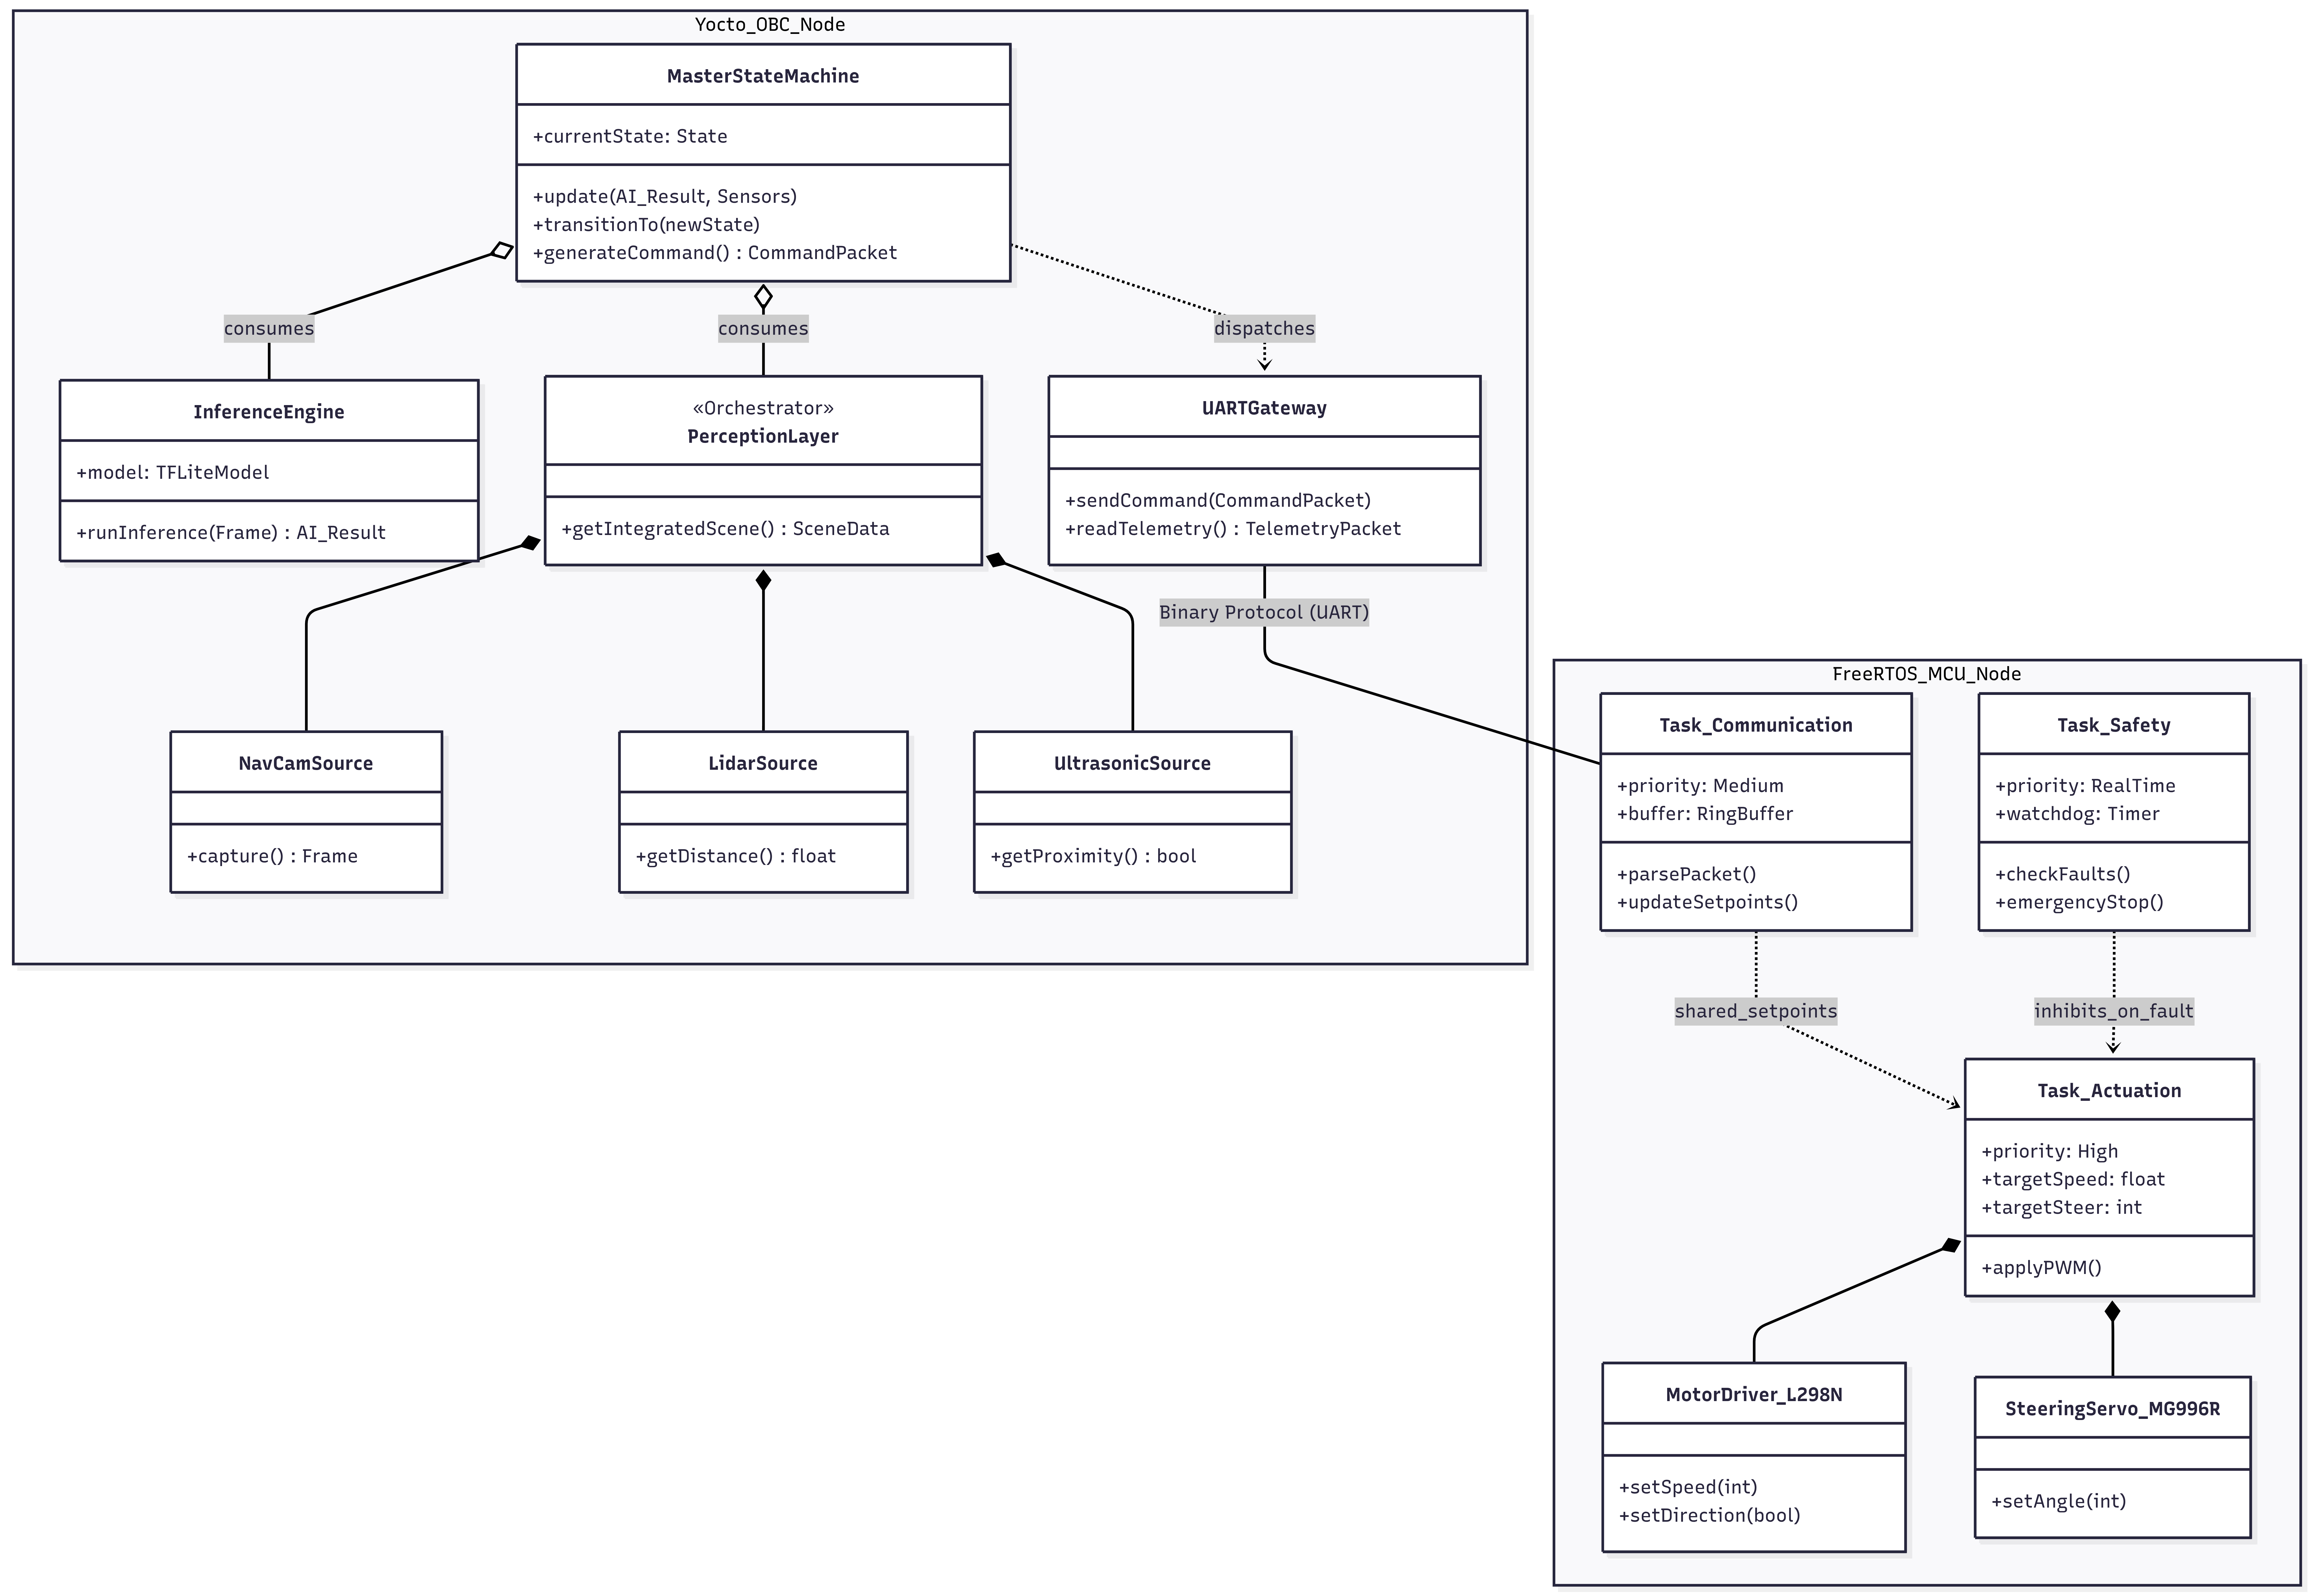
\includegraphics[width=0.7\paperheight]{figures/YoctoNodeImageProcessing.png}
    \caption{Vista funcional de la arquitectura de software: percepción + IA en Yocto (RPi5) y ejecución determinista en Rust \texttt{no\_std} bare-metal (Arduino Mega).}
    \label{fig:software_arqui}
\end{figure}
\end{landscape}

\subsubsection{Nodo A (Yocto/Linux): Percepción, IA y Máquina de Estados Maestra}
\label{subsubsec:nodoA_yocto}
La Raspberry Pi 5 ejecuta una imagen optimizada de \textbf{Yocto Project} (sin layers de ML genéricas, ver memoria de build limpio 2026-03-24) que centraliza la percepción de alto nivel de la \textbf{NavCam OV5647 (CSI)} y el \textbf{LiDAR TF02} (UART 115200\,bps). Los sensores de seguridad de corto rango (\textbf{HC-SR04} ultrasonido en GPIO y \textbf{VL53L0X} ToF en I2C) viven en el Nodo B (Arduino Mega) para mantener el lazo de \emph{emergency stop} fuera del camino crítico UART; sus lecturas llegan a la RPi5 sólo como telemetría agregada en los frames TLM.

El flujo de software en este nodo se divide en tres niveles:
\begin{enumerate}
    \item \textbf{Capa de Percepción:} Lectura directa de drivers del kernel (V4L2 para cámara CSI, UART para TF02) y consumo de telemetría del Nodo B vía CSP \texttt{csp\_if\_udp} (HC-SR04, VL53L0X, encoders, INA3221, ACS712 agregados).
    \item \textbf{Motor de Inferencia:} Ejecución del modelo \textbf{YOLOv8n-seg} (formato ONNX) para clasificación de transitabilidad y segmentación de obstáculos sobre los frames OV5647 (baseline COCO, $\sim$205\,ms/frame, $\sim$4.9\,FPS en RPi5 CPU; pendiente fine-tuning terreno volcánico --- RF-002).
    \item \textbf{Máquina de Estados Maestra (MSM, módulo \texttt{olympus\_hlc.msm}):} Gobierna el comportamiento global del rover basándose en los resultados de la IA y el estado de la misión. Dependiendo del estado activo (\texttt{STANDBY}, \texttt{EXPLORE}, \texttt{AVOID}, \texttt{RETREAT}, \texttt{CLIMB}, \texttt{FAULT}, \texttt{SAFE}), la MSM habilita o deshabilita subsistemas y genera los comandos ASCII para la MCU (\texttt{EXP:L:R}, \texttt{CLB:L:R}, \texttt{STB}, \texttt{RST}, \texttt{BNK:0}) según el ICD-LLC-001.
\end{enumerate}

\subsubsection{Nodo B (Rust \texttt{no\_std} bare-metal): Ejecución Determinista y Actuación}
\label{subsubsec:nodoB_freertos}
El Arduino Mega 2560 R3 ejecuta el firmware \textbf{\texttt{rover-low-level-controller}} (LLC v2.20) compilado con \textbf{Rust \texttt{no\_std} sobre \texttt{avr-hal}} y desplegado mediante \texttt{ravedude}; \textbf{no} usa un RTOS (FreeRTOS no aporta valor en esta plataforma AVR de 8\,bits dada la simplicidad del scheduler requerido). La determinación se logra con un \textbf{main loop cooperativo} de período fijo ($\sim$20\,ms) combinado con \textbf{interrupciones por hardware} para los caminos críticos, organizado en módulos:

\begin{itemize}
    \item \textbf{Módulo \texttt{comms} (USART0 con ISR FIFO):} Decodifica los frames ASCII entrantes desde la RPi5 (comandos \texttt{EXP/CLB/STB/RST/BNK:0/PING}) y emite telemetría \texttt{TLM:\dots} de vuelta. CRC opcional; integridad por handshake \texttt{PING$\rightarrow$PONG}.
    \item \textbf{Módulo \texttt{state\_machine} (MSM 7 estados + SafetyState paralelo):} Implementa los 7 estados \texttt{Standby/Explore/Avoid/Retreat/Climb/Fault/Safe} y la dimensión paralela \texttt{SafetyState (Normal/Warn/Limit/FaultStall)}. Gobierna las transiciones según sensores (HC-SR04 $<$200\,mm, TF02 $<$150\,mm, VL53L0X CLB $<$50\,mm, stall por encoders).
    \item \textbf{Módulo \texttt{motors} (\texttt{MotorWithEncoder}, drivers mixtos):} Genera PWM hacia los drivers \textbf{L298N (×1, FR/FL)} y \textbf{BTS7960 (×4, CR/CL/RR/RL)} usando la configuración mixed-drivers (commit \texttt{1845c4a}); aplica dead-band del 15\% y rampas; consume \texttt{QuadratureEncoder} fase A/B (D44--D49) para lazo cerrado por rueda.
    \item \textbf{Módulo \texttt{sensors}:} Drivers Rust para HC-SR04 (GPIO trigger/echo), VL53L0X (I2C 0x29), MPU-6050 (I2C 0x68), INA3221 (I2C bus-only, 3 canales), ACS712 (ADC analógico × 6) y TF02 (UART2 con fix FIFO en ISR USART2, commit \texttt{6dc27ec}).
    \item \textbf{Módulo \texttt{safety} (lazo de emergencia):} Verifica el watchdog UART contra la OBC, los umbrales \texttt{OC\_FAULT} de ACS712 (provisional 15\,A, pendiente calibración con \texttt{I\_stall} NFP-5840), las condiciones de stall por encoder y el corte de emergencia por sensores de corto rango. Una violación fuerza \texttt{state\_machine.transition\_to(Fault)} con \textit{paro seguro} en $\le$500\,ms (RF-005).
\end{itemize}

Cobertura de prueba en x86: 49/49 tests verdes (3 suites) al 2026-04-29. El despliegue en HW se realiza mediante \texttt{make flash-mixed PORT=/dev/ttyACM0}; la calibración de \texttt{OC\_FAULT\_BTS} con \texttt{I\_stall} medido en banco es prerrequisito antes de energizar BTS7960 con carga (procedimiento de 6 pasos, ver memoria \texttt{session\_2026\_04\_29\_llc\_protection}).

\subsubsection{Protocolo de Comunicación y Flujo de Mando}
\label{subsubsec:protocolo_serial}
El intercambio de información entre nodos se realiza mediante un protocolo binario ligero sobre el bus \textbf{UART}. La RPi 5 envía tramas que encapsulan el modo de operación y los parámetros de velocidad/dirección. A su vez, el Arduino reporta telemetría de bajo nivel (estado de motores, encoders y consumo energético del sensor INA219). Esta separación asegura que el cómputo pesado de IA no interfiera con el determinismo requerido para el control de los motores.
En resumen, el Nodo A ejecuta el pipeline de visión e inferencia, empaqueta resultados en un payload binario compacto y los transmite por un enlace ligero. El Nodo B transforma dichos payloads en eventos internos del MAS, los distribuye mediante un broker de mensajes y, a través de agentes especializados, decide acciones, opera actuadores y mantiene telemetría/monitoreo. Esta partición mejora la escalabilidad (IA y control desacoplados), facilita la verificación del comportamiento en tiempo real en el MCU y permite evolucionar agentes y modelos de IA de forma independiente.
